\documentclass[preprint]{sigplanconf}

\usepackage{amssymb}
\usepackage{amsthm}
\usepackage{breakurl}             % Not needed if you use pdflatex only.
\usepackage{color}
\usepackage{epsfig}
\usepackage{esvect}
\usepackage{listings}
\usepackage{mathpartir}
\usepackage{MnSymbol}
\usepackage{multirow}
\usepackage{rotating}

\lstdefinestyle{Caml}{language=Caml,%
  literate={when}{{{\bf when}}}4
}

\lstdefinestyle{C++}{language=C++,%
showstringspaces=false,
  columns=fullflexible,
  escapechar=@,
  basicstyle=\sffamily,
%  commentstyle=\rmfamily\itshape,
  moredelim=**[is][\color{white}]{~}{~},
  literate={[<]}{{\textless}}1      {[>]}{{\textgreater}}1 %
           {<}{{$\langle$}}1        {>}{{$\rangle$}}1 %
           {<=}{{$\leq$}}1          {>=}{{$\geq$}}1          
           {==}{{$==$}}2            {!=}{{$\neq$}}1 %
           {=>}{{$\Rightarrow\;$}}1 {->}{{$\rightarrow{}$}}1 %
           {<:}{{$\subtype{}\ $}}1  {<-}{{$\leftarrow$}}1 %
           {e1}{{$e_1$}}2 {e2}{{$e_2$}}2 {e3}{{$e_3$}}2 {e4}{{$e_4$}}2%
           {E1}{{$E_1$}}2 {E2}{{$E_2$}}2 {E3}{{$E_3$}}2 {E4}{{$E_4$}}2%
           {m_e1}{{$m\_e_1$}}4 {m_e2}{{$m\_e_2$}}4 {m_e3}{{$m\_e_3$}}4 {m_e4}{{$m\_e_4$}}4%
           {Match}{{\emph{Match}}}5 %
           {Case}{{\emph{Case}}}4 %
           {Que}{{\emph{Que}}}3 %
           {Otherwise}{{\emph{Otherwise}}}9 %
           {EndMatch}{{\emph{EndMatch}}}8 %
           {CM}{{\emph{CM}}}2 {KS}{{\emph{KS}}}2 {KV}{{\emph{KV}}}2 
}
\lstset{style=C++}
\DeclareRobustCommand{\code}[1]{{\lstinline[breaklines=false,escapechar=@]{#1}}}
\DeclareRobustCommand{\codehaskell}[1]{{\lstinline[breaklines=false,language=Haskell]{#1}}}
\DeclareRobustCommand{\codeocaml}[1]{{\lstinline[breaklines=false,language=Caml]{#1}}}

\newtheorem{theorem}{Theorem}
\newtheorem{corollary}{Corollary}

%% grammar commands
\newcommand{\Rule}[1]{{\rmfamily\itshape{#1}}}
\newcommand{\Alt}{\ensuremath{|}}
\newcommand{\is}{$::=$}
\newcommand{\subtype}{\textless:}
\newcommand{\evals}{\Rightarrow}
\newcommand{\evalspp}{\Rightarrow^+}
\newcommand{\DynCast}[2]{\ensuremath{dc\langle{#1}\rangle({#2})}}
\newcommand{\nullptr}{\ensuremath{\bot}}

\newcommand{\f}[1]{{ {\bf \textcolor{blue}{#1\%}}}}
\newcommand{\s}[1]{{ {\em \textcolor{cyan}{#1\%}}}}
\newcommand{\n}[1]{{ {\bf ~ ~ ~ ~ }}}
\newcommand{\Opn}{{\scriptsize {\bf Open}}}
\newcommand{\Cls}{{\scriptsize {\bf Tag}}}
\newcommand{\Unn}{{\scriptsize {\bf Union}}}

%\newcommand{\gwNGPp}{\n{}}
%\newcommand{\gwNGKp}{\n{}}
 \newcommand{\gwNGUp}{\n{}}
%\newcommand{\gwNSPp}{\n{}}
%\newcommand{\gwNSKp}{\n{}}
 \newcommand{\gwNSUp}{\n{}}
%\newcommand{\vwNGPp}{\n{}}
%\newcommand{\vwNGKp}{\n{}}
 \newcommand{\vwNGUp}{\n{}}
%\newcommand{\vwNSPp}{\n{}}
%\newcommand{\vwNSKp}{\n{}}
 \newcommand{\vwNSUp}{\n{}}
%\newcommand{\vxNGPp}{\n{}}
%\newcommand{\vxNGKp}{\n{}}
 \newcommand{\vxNGUp}{\n{}}
%\newcommand{\vxNSPp}{\n{}}
%\newcommand{\vxNSKp}{\n{}}
 \newcommand{\vxNSUp}{\n{}}

%\newcommand{\gwNGPq}{\n{}}
%\newcommand{\gwNGKq}{\n{}}
 \newcommand{\gwNGUq}{\n{}}
%\newcommand{\gwNSPq}{\n{}}
%\newcommand{\gwNSKq}{\n{}}
 \newcommand{\gwNSUq}{\n{}}
%\newcommand{\vwNGPq}{\n{}}
%\newcommand{\vwNGKq}{\n{}}
 \newcommand{\vwNGUq}{\n{}}
%\newcommand{\vwNSPq}{\n{}}
%\newcommand{\vwNSKq}{\n{}}
 \newcommand{\vwNSUq}{\n{}}
%\newcommand{\vxNGPq}{\n{}}
%\newcommand{\vxNGKq}{\n{}}
 \newcommand{\vxNGUq}{\n{}}
%\newcommand{\vxNSPq}{\n{}}
%\newcommand{\vxNSKq}{\n{}}
 \newcommand{\vxNSUq}{\n{}}

%\newcommand{\gwNGPn}{\n{}}
%\newcommand{\gwNGKn}{\n{}}
 \newcommand{\gwNGUn}{\n{}}
%\newcommand{\gwNSPn}{\n{}}
%\newcommand{\gwNSKn}{\n{}}
 \newcommand{\gwNSUn}{\n{}}
%\newcommand{\vwNGPn}{\n{}}
%\newcommand{\vwNGKn}{\n{}}
 \newcommand{\vwNGUn}{\n{}}
%\newcommand{\vwNSPn}{\n{}}
%\newcommand{\vwNSKn}{\n{}}
 \newcommand{\vwNSUn}{\n{}}
%\newcommand{\vxNGPn}{\n{}}
%\newcommand{\vxNGKn}{\n{}}
 \newcommand{\vxNGUn}{\n{}}
%\newcommand{\vxNSPn}{\n{}}
%\newcommand{\vxNSKn}{\n{}}
 \newcommand{\vxNSUn}{\n{}}


%\newcommand{\gwYGPp}{\n{}}
 \newcommand{\gwYGKp}{\n{}}
 \newcommand{\gwYGUp}{\n{}}
%\newcommand{\gwYSPp}{\n{}}
 \newcommand{\gwYSKp}{\n{}}
 \newcommand{\gwYSUp}{\n{}}
%\newcommand{\vwYGPp}{\n{}}
 \newcommand{\vwYGKp}{\n{}}
 \newcommand{\vwYGUp}{\n{}}
%\newcommand{\vwYSPp}{\n{}}
 \newcommand{\vwYSKp}{\n{}}
 \newcommand{\vwYSUp}{\n{}}
%\newcommand{\vxYGPp}{\n{}}
 \newcommand{\vxYGKp}{\n{}}
 \newcommand{\vxYGUp}{\n{}}
%\newcommand{\vxYSPp}{\n{}}
 \newcommand{\vxYSKp}{\n{}}
 \newcommand{\vxYSUp}{\n{}}

%\newcommand{\gwYGPq}{\n{}}
 \newcommand{\gwYGKq}{\n{}}
 \newcommand{\gwYGUq}{\n{}}
%\newcommand{\gwYSPq}{\n{}}
 \newcommand{\gwYSKq}{\n{}}
 \newcommand{\gwYSUq}{\n{}}
%\newcommand{\vwYGPq}{\n{}}
 \newcommand{\vwYGKq}{\n{}}
 \newcommand{\vwYGUq}{\n{}}
%\newcommand{\vwYSPq}{\n{}}
 \newcommand{\vwYSKq}{\n{}}
 \newcommand{\vwYSUq}{\n{}}
%\newcommand{\vxYGPq}{\n{}}
 \newcommand{\vxYGKq}{\n{}}
 \newcommand{\vxYGUq}{\n{}}
%\newcommand{\vxYSPq}{\n{}}
 \newcommand{\vxYSKq}{\n{}}
 \newcommand{\vxYSUq}{\n{}}

%\newcommand{\gwYGPn}{\n{}}
 \newcommand{\gwYGKn}{\n{}}
 \newcommand{\gwYGUn}{\n{}}
%\newcommand{\gwYSPn}{\n{}}
 \newcommand{\gwYSKn}{\n{}}
 \newcommand{\gwYSUn}{\n{}}
%\newcommand{\vwYGPn}{\n{}}
 \newcommand{\vwYGKn}{\n{}}
 \newcommand{\vwYGUn}{\n{}}
%\newcommand{\vwYSPn}{\n{}}
 \newcommand{\vwYSKn}{\n{}}
 \newcommand{\vwYSUn}{\n{}}
%\newcommand{\vxYGPn}{\n{}}
 \newcommand{\vxYGKn}{\n{}}
 \newcommand{\vxYGUn}{\n{}}
%\newcommand{\vxYSPn}{\n{}}
 \newcommand{\vxYSKn}{\n{}}
 \newcommand{\vxYSUn}{\n{}}

 \newcommand{\GwNGPp}{\n{}}
 \newcommand{\GwNGKp}{\n{}}
 \newcommand{\GwNGUp}{\n{}}
 \newcommand{\GwNSPp}{\n{}}
 \newcommand{\GwNSKp}{\n{}}
 \newcommand{\GwNSUp}{\n{}}
%\newcommand{\VwNGPp}{\n{}}
%\newcommand{\VwNGKp}{\n{}}
 \newcommand{\VwNGUp}{\n{}}
%\newcommand{\VwNSPp}{\n{}}
%\newcommand{\VwNSKp}{\n{}}
 \newcommand{\VwNSUp}{\n{}}
%\newcommand{\VxNGPp}{\n{}}
%\newcommand{\VxNGKp}{\n{}}
 \newcommand{\VxNGUp}{\n{}}
%\newcommand{\VxNSPp}{\n{}}
%\newcommand{\VxNSKp}{\n{}}
 \newcommand{\VxNSUp}{\n{}}

 \newcommand{\GwNGPq}{\n{}}
 \newcommand{\GwNGKq}{\n{}}
 \newcommand{\GwNGUq}{\n{}}
 \newcommand{\GwNSPq}{\n{}}
 \newcommand{\GwNSKq}{\n{}}
 \newcommand{\GwNSUq}{\n{}}
%\newcommand{\VwNGPq}{\n{}}
%\newcommand{\VwNGKq}{\n{}}
 \newcommand{\VwNGUq}{\n{}}
%\newcommand{\VwNSPq}{\n{}}
%\newcommand{\VwNSKq}{\n{}}
 \newcommand{\VwNSUq}{\n{}}
%\newcommand{\VxNGPq}{\n{}}
%\newcommand{\VxNGKq}{\n{}}
 \newcommand{\VxNGUq}{\n{}}
%\newcommand{\VxNSPq}{\n{}}
%\newcommand{\VxNSKq}{\n{}}
 \newcommand{\VxNSUq}{\n{}}

 \newcommand{\GwNGPn}{\n{}}
 \newcommand{\GwNGKn}{\n{}}
 \newcommand{\GwNGUn}{\n{}}
 \newcommand{\GwNSPn}{\n{}}
 \newcommand{\GwNSKn}{\n{}}
 \newcommand{\GwNSUn}{\n{}}
%\newcommand{\VwNGPn}{\n{}}
%\newcommand{\VwNGKn}{\n{}}
 \newcommand{\VwNGUn}{\n{}}
%\newcommand{\VwNSPn}{\n{}}
%\newcommand{\VwNSKn}{\n{}}
 \newcommand{\VwNSUn}{\n{}}
%\newcommand{\VxNGPn}{\n{}}
%\newcommand{\VxNGKn}{\n{}}
 \newcommand{\VxNGUn}{\n{}}
%\newcommand{\VxNSPn}{\n{}}
%\newcommand{\VxNSKn}{\n{}}
 \newcommand{\VxNSUn}{\n{}}


 \newcommand{\GwYGPp}{\n{}}
 \newcommand{\GwYGKp}{\n{}}
 \newcommand{\GwYGUp}{\n{}}
 \newcommand{\GwYSPp}{\n{}}
 \newcommand{\GwYSKp}{\n{}}
 \newcommand{\GwYSUp}{\n{}}
%\newcommand{\VwYGPp}{\n{}}
 \newcommand{\VwYGKp}{\n{}}
 \newcommand{\VwYGUp}{\n{}}
%\newcommand{\VwYSPp}{\n{}}
 \newcommand{\VwYSKp}{\n{}}
 \newcommand{\VwYSUp}{\n{}}
%\newcommand{\VxYGPp}{\n{}}
 \newcommand{\VxYGKp}{\n{}}
 \newcommand{\VxYGUp}{\n{}}
%\newcommand{\VxYSPp}{\n{}}
 \newcommand{\VxYSKp}{\n{}}
 \newcommand{\VxYSUp}{\n{}}

 \newcommand{\GwYGPq}{\n{}}
 \newcommand{\GwYGKq}{\n{}}
 \newcommand{\GwYGUq}{\n{}}
 \newcommand{\GwYSPq}{\n{}}
 \newcommand{\GwYSKq}{\n{}}
 \newcommand{\GwYSUq}{\n{}}
%\newcommand{\VwYGPq}{\n{}}
 \newcommand{\VwYGKq}{\n{}}
 \newcommand{\VwYGUq}{\n{}}
%\newcommand{\VwYSPq}{\n{}}
 \newcommand{\VwYSKq}{\n{}}
 \newcommand{\VwYSUq}{\n{}}
%\newcommand{\VxYGPq}{\n{}}
 \newcommand{\VxYGKq}{\n{}}
 \newcommand{\VxYGUq}{\n{}}
%\newcommand{\VxYSPq}{\n{}}
 \newcommand{\VxYSKq}{\n{}}
 \newcommand{\VxYSUq}{\n{}}

 \newcommand{\GwYGPn}{\n{}}
 \newcommand{\GwYGKn}{\n{}}
 \newcommand{\GwYGUn}{\n{}}
 \newcommand{\GwYSPn}{\n{}}
 \newcommand{\GwYSKn}{\n{}}
 \newcommand{\GwYSUn}{\n{}}
%\newcommand{\VwYGPn}{\n{}}
 \newcommand{\VwYGKn}{\n{}}
 \newcommand{\VwYGUn}{\n{}}
%\newcommand{\VwYSPn}{\n{}}
 \newcommand{\VwYSKn}{\n{}}
 \newcommand{\VwYSUn}{\n{}}
%\newcommand{\VxYGPn}{\n{}}
 \newcommand{\VxYGKn}{\n{}}
 \newcommand{\VxYGUn}{\n{}}
%\newcommand{\VxYSPn}{\n{}}
 \newcommand{\VxYSKn}{\n{}}
 \newcommand{\VxYSUn}{\n{}}

% This file defines variables with performance numbers for the table in Evaluation section 
\newcommand{\vwYGPp}{\f{2}} 
\newcommand{\vwYGPn}{\f{1}} 
\newcommand{\vwYGPq}{\s{7}} 
\newcommand{\vwYSPp}{\f{4}} 
\newcommand{\vwYSPn}{\f{4}} 
\newcommand{\vwYSPq}{\f{133}} 
\newcommand{\vwNGKp}{\f{131}} 
\newcommand{\vwNGKn}{\f{25}} 
\newcommand{\vwNGKq}{\f{61}} 
\newcommand{\vwNGPp}{\s{2}} 
\newcommand{\vwNGPn}{\s{5}} 
\newcommand{\vwNGPq}{\s{10}} 
\newcommand{\vwNSKp}{\f{110}} 
\newcommand{\vwNSKn}{\f{25}} 
\newcommand{\vwNSKq}{\f{59}} 
\newcommand{\vwNSPp}{\s{4}} 
\newcommand{\vwNSPn}{\s{9}} 
\newcommand{\vwNSPq}{\s{14}} 
\newcommand{\vxYGPp}{\f{6}} 
\newcommand{\vxYGPn}{\s{15}} 
\newcommand{\vxYGPq}{\f{134}} 
\newcommand{\vxYSPp}{\s{6}} 
\newcommand{\vxYSPn}{\s{20}} 
\newcommand{\vxYSPq}{\f{121}} 
\newcommand{\vxNGKp}{\f{55}} 
\newcommand{\vxNGKn}{\f{9}} 
\newcommand{\vxNGKq}{\f{2}} 
\newcommand{\vxNGPp}{\s{0}} 
\newcommand{\vxNGPn}{\s{34}} 
\newcommand{\vxNGPq}{\s{29}} 
\newcommand{\vxNSKp}{\f{55}} 
\newcommand{\vxNSKn}{\f{12}} 
\newcommand{\vxNSKq}{\f{3}} 
\newcommand{\vxNSPp}{\s{28}} 
\newcommand{\vxNSPn}{\s{31}} 
\newcommand{\vxNSPq}{\s{38}} 
\newcommand{\VwYGPp}{\f{43}} 
\newcommand{\VwYGPn}{\f{4}} 
\newcommand{\VwYGPq}{\f{156}} 
\newcommand{\VwYSPp}{\f{39}} 
\newcommand{\VwYSPn}{\f{7}} 
\newcommand{\VwYSPq}{\f{176}} 
\newcommand{\VwNGKp}{\f{121}} 
\newcommand{\VwNGKn}{\f{38}} 
\newcommand{\VwNGKq}{\f{32}} 
\newcommand{\VwNGPp}{\f{41}} 
\newcommand{\VwNGPn}{\s{10}} 
\newcommand{\VwNGPq}{\f{12}} 
\newcommand{\VwNSKp}{\f{149}} 
\newcommand{\VwNSKn}{\f{43}} 
\newcommand{\VwNSKq}{\f{34}} 
\newcommand{\VwNSPp}{\f{42}} 
\newcommand{\VwNSPn}{\s{12}} 
\newcommand{\VwNSPq}{\f{3}} 
\newcommand{\VxYGPp}{\f{2}} 
\newcommand{\VxYGPn}{\s{6}} 
\newcommand{\VxYGPq}{\f{125}} 
\newcommand{\VxYSPp}{\s{0}} 
\newcommand{\VxYSPn}{\s{7}} 
\newcommand{\VxYSPq}{\f{136}} 
\newcommand{\VxNGKp}{\f{76}} 
\newcommand{\VxNGKn}{\f{17}} 
\newcommand{\VxNGKq}{\f{11}} 
\newcommand{\VxNGPp}{\s{6}} 
\newcommand{\VxNGPn}{\s{22}} 
\newcommand{\VxNGPq}{\s{26}} 
\newcommand{\VxNSKp}{\f{76}} 
\newcommand{\VxNSKn}{\f{17}} 
\newcommand{\VxNSKq}{\f{14}} 
\newcommand{\VxNSPp}{\f{11}} 
\newcommand{\VxNSPn}{\s{19}} 
\newcommand{\VxNSPq}{\s{5}} 

%%%%%%%%%%%%%%%%%%%%%%%%%%%%%%%%%%%%%%%%%%%%%%%%%%%%%%%%%%%%%%%%%%%%%%%%%%%%%%%%%%%

%\newcommand{\vwYGPp}{\f{2}}
%\newcommand{\vwYGPn}{\f{1}}
%\newcommand{\vwYGPq}{\s{7}}
%\newcommand{\vwYSPp}{\f{4}}
%\newcommand{\vwYSPn}{\f{4}}
%\newcommand{\vwYSPq}{\f{133}}
%\newcommand{\vwNGKp}{\f{131}}
%\newcommand{\vwNGKn}{\f{25}}
%\newcommand{\vwNGKq}{\f{61}}
%\newcommand{\vwNGPp}{\s{2}}
%\newcommand{\vwNGPn}{\s{5}}
%\newcommand{\vwNGPq}{\s{10}}
%\newcommand{\vwNSKp}{\f{108}}
%\newcommand{\vwNSKn}{\f{25}}
%\newcommand{\vwNSKq}{\f{59}}
%\newcommand{\vwNSPp}{\s{4}}
%\newcommand{\vwNSPn}{\s{9}}
%\newcommand{\vwNSPq}{\s{13}}
%\newcommand{\vxYGPp}{\f{6}}
%\newcommand{\vxYGPn}{\s{15}}
%\newcommand{\vxYGPq}{\f{134}}
%\newcommand{\vxYSPp}{\s{6}}
%\newcommand{\vxYSPn}{\s{20}}
%\newcommand{\vxYSPq}{\f{122}}
%\newcommand{\vxNGKp}{\f{55}}
%\newcommand{\vxNGKn}{\f{9}}
%\newcommand{\vxNGKq}{\f{2}}
%\newcommand{\vxNGPp}{\s{0}}
%\newcommand{\vxNGPn}{\s{34}}
%\newcommand{\vxNGPq}{\s{29}}
%\newcommand{\vxNSKp}{\f{55}}
%\newcommand{\vxNSKn}{\f{12}}
%\newcommand{\vxNSKq}{\f{3}}
%\newcommand{\vxNSPp}{\s{28}}
%\newcommand{\vxNSPn}{\s{31}}
%\newcommand{\vxNSPq}{\s{37}}

\newcommand{\gwYGPp}{\f{105}}
\newcommand{\gwYGPn}{\f{28}}
\newcommand{\gwYGPq}{\f{59}}
\newcommand{\gwYSPp}{\f{119}}
\newcommand{\gwYSPn}{\f{22}}
\newcommand{\gwYSPq}{\f{272}}
\newcommand{\gwNGKp}{\f{329}}
\newcommand{\gwNGKn}{\f{531}}
\newcommand{\gwNGKq}{\f{522}}
\newcommand{\gwNGPp}{\f{85}}
\newcommand{\gwNGPn}{\f{7}}
\newcommand{\gwNGPq}{\f{15}}
\newcommand{\gwNSKp}{\f{274}}
\newcommand{\gwNSKn}{\f{537}}
\newcommand{\gwNSKq}{\f{528}}
\newcommand{\gwNSPp}{\f{89}}
\newcommand{\gwNSPn}{\f{8}}
\newcommand{\gwNSPq}{\f{18}}


\newsavebox{\sembox}
\newlength{\semwidth}
\newlength{\boxwidth}

\newcommand{\Sem}[1]{%
\sbox{\sembox}{\ensuremath{#1}}%
\settowidth{\semwidth}{\usebox{\sembox}}%
\sbox{\sembox}{\ensuremath{\left[\usebox{\sembox}\right]}}%
\settowidth{\boxwidth}{\usebox{\sembox}}%
\addtolength{\boxwidth}{-\semwidth}%
\left[\hspace{-0.3\boxwidth}%
\usebox{\sembox}%
\hspace{-0.3\boxwidth}\right]%
}

\newcommand{\authormodification}[2]{{\color{#1}#2}}
\newcommand{\ys}[1]{\authormodification{blue}{#1}}
\newcommand{\bs}[1]{\authormodification{red}{#1}}
\newcommand{\gdr}[1]{\authormodification{magenta}{#1}}

\begin{document}

%\conferenceinfo{DSL 2011}{Bordeaux, France} 
%\copyrightyear{2011} 
%\copyrightdata{[to be supplied]} 

\titlebanner{Technical Report}        % These are ignored unless
\preprintfooter{Y.Solodkyy, G.Dos Reis, B.Stroustrup: Pattern Matching for C++}   % 'preprint' option specified.

\title{Pattern Matching for C++}
\subtitle{your \code{visit}, Jim, is not \code{accept}able anymore}

\authorinfo{Yuriy Solodkyy\and Gabriel Dos Reis\and Bjarne Stroustrup}
           {Texas A\&M University\\ Texas, USA}
           {\{yuriys,gdr,bs\}@cse.tamu.edu}

\maketitle

\begin{abstract}
Pattern matching has been known in functional programming community as an 
abstraction mechanism that greatly simplifies the code. Following the success of 
functional languages, several imperative programming languages had introduced 
pattern matching into them. While this is relatively easy to do a-priori, when 
designing a new language, this might become quite a challenge to do a-posteriori 
when trying to introduce it into an industry strength language like C++. We 
present functional style pattern matching for C++ implemented as a library. 
Depending on a use case, our solution matches or outperforms its de facto 
contender -- the visitor design pattern, traditionally used in pattern-matching 
scenarios in C++. Unlike the visitor pattern, our solution is non-intrusive, 
open to new classes, avoids the control inversion and is much more concise, 
easier to read, maintain and comprehend. It also mimics many of the pattern 
matching facilities available in other languages on the first class basis, 
letting us experiment with them without any changes to the compiler. The 
solution can be reused in other object-oriented languages to implement
\emph{type switching}, \emph{type testing}, \emph{pattern matching} and 
\emph{multiple dispatch} efficiently.
\end{abstract}

\category{CR-number}{subcategory}{third-level}

\terms
Languages, Design

\keywords
Pattern Matching, Visitor Design Pattern, Expression Problem, C++

\section{Introduction} %%%%%%%%%%%%%%%%%%%%%%%%%%%%%%%%%%%%%%%%%%%%%%%%%%%%%%%%%
\label{sec:intro}

%Motivate the problem
%Give a summary of the paper: what you did and how
%Explicitly state your contribution

%From Cardelli: Compiling a Functional Language
%Pattern matching communicates highly structured information
%about the input parameters. As a consequence, a compiler can produce better code from a pattern
%matching description than from a corresponding sequence of discrimination and selection
%operations.
%
%ML pattern matching is less powerful than, for example, Prolog pattern matching, because
%every variable can occur only once in an ML pattern. Hence, ML pattern matching is just an
%abbreviation for nested if-then-else, case statements and selection functions.


Pattern matching is an abstraction supported by many programming languages, which 
allows the user to describe in a breve manner a (possibly infinite) set of 
values accepted by the pattern. Pattern represents effectively a predicate on 
values, and is usually expected to be much more concise and readable than the 
equivalent predicate spelled out directly.

Popularized by functional programming community, most notably Hope\cite{BMS80}, 
ML\cite{ML90}, Miranda\cite{Miranda85} and Haskell\cite{Haskell98Book}, for 
providing syntax very close to mathematical notations, pattern matching has 
since been making its way into many imperative programming languages like 
Pizza\cite{Odersky97pizzainto}, Scala\cite{Scala2nd}, Fortress\cite{RPS10}, 
Java\cite{Liu03jmatch:iterable,HydroJ2003}, C++\cite{Prop96}, 
Eiffel\cite{Moreau:2003} and others. While this is relatively
easy to do a-priori when designing a new language, the introduction of pattern 
matching into an industry strengths language a-posteriori might become a 
challenge. The obvious utility of the feature may be overshadowed by the 
complications in the language semantics necessary to make pattern matching work 
with other features of the language. A prototype implementation will likely 
require a lot of effort, but will be hard to publish due to lack of novelty.

To balance the utility and effort we decided to start with a Semantically 
Enhanced Library Language (SELL) approach\cite{SELL}, that promotes subsetting a
general-purpose programming language with a library, extended with a tool 
support. This will typically not provide you 100\% of the functionality that a 
language extension would do, but will rather give you 80\% of it at 20\% of the 
time. This turned out to be an economic decision as we ended up not requiring 
any external tool support at all, while providing a descent level of convenience 
and a great performance.

Naturally, our library-only solution has limitations and inconveniencies that 
stem from the fact that we work in a SELL setting. We are certain, however, that 
those can be easily overcome in a language solution and we provide relevant 
discussions when necessary. We regard our current solution as a proof of  
concept that sets the minimum threshold for performance, brevity, clarity and 
usefulness of the ultimate language solution for pattern matching in C++. It is 
a fully functional transitional facility, that lets users experiment with 
pattern matching in C++, while letting us experiment with and eventually shape 
the language solution.

To give a quick taste of what our library enables, let us look at an example from 
the domain where pattern matching is known to cut the edge of laconism and 
clarity -- compiler construction. Imagine a simple language of expressions:

\begin{lstlisting}
@$exp$ \is{} $val$ \Alt{} $exp+exp$ \Alt{} $exp-exp$ \Alt{} $exp*exp$ \Alt{} $exp/exp$@
\end{lstlisting}

OCaml data type describing this grammar as well as simple evaluator of expressions 
in it can be declared as following:

\begin{lstlisting}[language=Caml,keepspaces,columns=flexible]
type expr = Value  of int
          | Plus   of expr * expr
          | Minus  of expr * expr
          | Times  of expr * expr
          | Divide of expr * expr
          ;;

let rec eval e =
  match e with
            Value  v      -> v
          | Plus   (a, b) -> (eval a) + (eval b)
          | Minus  (a, b) -> (eval a) - (eval b)
          | Times  (a, b) -> (eval a) * (eval b)
          | Divide (a, b) -> (eval a) / (eval b)
          ;;
\end{lstlisting}

The corresponding C++ data types are slightly more verbose, though the only 
reason we have not parameterized them was to keep the example simple.

\begin{lstlisting}[keepspaces,columns=flexible]
struct Expr { virtual @$\sim$@Expr() {} };
struct Value  : Expr { int value; };
struct Plus   : Expr { Expr* exp1; Expr* exp2; };
struct Minus  : Expr { Expr* exp1; Expr* exp2; };
struct Times  : Expr { Expr* exp1; Expr* exp2; };
struct Divide : Expr { Expr* exp1; Expr* exp2; };
\end{lstlisting}

Together with evaluator presented below, they form an instance of the 
\emph{Interpreter Design Pattern}\cite{DesignPatterns1993}. Unlike the type 
definitions, the evaluator for the language, implemented on top of our pattern 
matching library is almost as laconic as its version in OCaml:

\begin{lstlisting}[keepspaces,columns=flexible]
int eval(const Expr* e)
{
    Match(e)@\footnote{We use alternative formatting on symbols representing preprocessor macros}@
    {
        Case(Value,  n)    return n;
        Case(Plus,   a, b) return eval(a) + eval(b);
        Case(Minus,  a, b) return eval(a) - eval(b);
        Case(Times,  a, b) return eval(a) * eval(b);
        Case(Divide, a, b) return eval(a) / eval(b);
    }
    EndMatch
}
\end{lstlisting}

The only definitions we omitted here that prevent the example from being fully 
functional are the mappings of binding positions to corresponding class members. 
We list them here for completeness, while their meaning will be explained later 
in section~\ref{sec:bnd}. Here we would like to mention though that these 
definitions are only needed to support the variables binding and not the type 
switching functionality of the \code{Match}.

\begin{lstlisting}[keepspaces,columns=flexible]
template <> struct bindings<Value>  { CM(0,Value::value); };
template <> struct bindings<Plus>   { CM(0,Plus::exp1); 
  ...                                 CM(1,Plus::exp2);   };
template <> struct bindings<Divide> { CM(0,Divide::exp1); 
                                      CM(1,Divide::exp2); };
\end{lstlisting}

The above syntax is enabled without any external tool support using new C++0x 
features\cite{C++0x}, template meta-programming and macros. As we 
show in section~\ref{sec:eval}, it runs up to 80\% faster (depending on the usage 
scenario, compiler and underlain hardware) than a similar code crafted with the 
\emph{Visitor Design Pattern}.

\subsection{Motivation}

%\subsection{Excursus}

The ideas and the library presented here originated from our rather 
unsatisfactory experience in working with various C++ front-ends and program 
analysis frameworks developed in C++\cite{Pivot09,Phoenix,Clang,Lise}. The 
problem was not in the frameworks per se, but in the fact that we had to use 
\emph{Visitor Design Pattern}\cite{DesignPatterns1993} to inspect, traverse and 
elaborate abstract syntax trees of their target languages. Having written enough 
visitors to realize how unsuitable they were for the job, we started looking for 
other mechanisms to work with abstract syntax trees, even if they would have 
turned out to be significantly slower. 
Presence of dynamic casts in many places, often nested, to answer simple 
structural questions without having to resort to visitors, was a strong 
indicator that even though visitors were fast, in many non-critical cases 
users preferred shorter, cleaner and a more clear code to performance.
The usage of \code{dynamic\_cast} in those cases resembled the use of 
pattern matching in functional languages to unpack algebraic data types. 
Functional languages have been long known to be very suitable for developing 
program analysis tools because of the brevity with which the necessary 
algorithms can be expressed. This is why our initial goal was to develop a 
domain-specific library within C++ that would enable us to express various 
predicates on tree-like structures with the laconism of functional languages.

%[From Emir PhD Thesis 1.3]
%In the context of the JAVA virtual machine (and any other object system that supports runtime
%type information), a much more direct way of obtaining the dynamic type of a value is
%to use an instanceof-check. Although these are considered bad style, programmers make
%use of them frequently, in order to avoid the overhead of using a Visitor implementation.
%They are error prone since it is possible to perform a cast without a preceding check.

\subsection{Expression Problem}

Functional languages allow for easy addition of new functions on existing data 
types, but fall short in extending data types themselves (e.g. with new constructors), 
which requires modifying the source code. Object-oriented languages, on the 
other hand, make data type extension trivial through inheritance, but addition 
of new functions that work on these classes typically requires changes to class 
definition. This dilema was first discussed by Cook\cite{Cook90} and then 
accentuated by Wadler\cite{exprproblem} under the name \emph{expression problem} 
he coined. Quoting Wadler:

\emph{``The Expression Problem is a new name for an old problem. The goal is
to define a datatype by cases, where one can add new cases to the
datatype and new functions over the datatype, without recompiling
existing code, and while retaining static type safety (e.g., no
casts)''}.

Zenger and Odersky later refined the problem in the context of independently 
extensible solutions\cite{fool12} as a challenge to find an implementation 
technique which satisfies the following requirements:

\begin{itemize}
\item Extensibility in both dimensions: It should be possible to add new data 
      variants, while adapting the existing operations accordingly. It should 
      also be possible to introduce new functions.
\item Strong static type safety: It should be impossible to apply a function to 
      a data variant, which it cannot handle.
\item No modification or duplication: Existing code should neither be modified 
      nor duplicated.
\item Separate compilation: Neither datatype extensions nor addition of new 
      functions should require re-typechecking the original datatype or 
      existing functions. No safety checks should be deferred until link or 
      runtime.
\item Independent extensibility: It should be possible to combine independently 
      developed extensions so that they can be used jointly.
\end{itemize}

%Paraphrasing, the expression problem can be summarized as a problem of 
%supporting modular extensibility of both data and functions at the same time in 
%one programming language.

Numerous solutions have been proposed to dealing with expression problem in both 
functional and object-oriented camps, but notably very few satisfy all of the 
above requirements. We refer the reader to Zenger and Odersky's original 
manuscript for discussion of the approaches\cite{fool12}. Interestingly, most of 
the discussed object-oriented solutions were focusing on the visitor design 
pattern, which even today seems to be the most commonly used approach to dealing 
with expression problem in practice.

\subsection{Visitor Design Pattern}
\label{sec:vdp}

%Discuss visitor design pattern and its problems.
%\begin{itemize}
%\item Intrusive - requires changes to the hierarchy
%\item Not open  - addition of new classes changes visitor interface
%\item Does not provide by default relation between visitors of base and derived classes
%\item Control inversion
%\item Cannot be generically extended to handling n arguments
%\end{itemize}

%[From Extensible Algebraic Datatypes with Defaults]
%In the object-oriented approach, data is modelled by a set of classes, sharing 
%a common interface. Each subclass defines its own implementation of eval. Whereas
%extending the datatype with new variants is simply done by
%creating new classes, adding new operations involves modifications
%of the abstract base class.

\emph{Visitor Design Pattern}\cite{DesignPatterns1993} was devised to solve a problem 
of extending existing classes with new functions in object-oriented languages. 
Consider the above Expr example and imagine we would like to provide a pretty 
printing of expressions. A typical object-oriented approach would be to 
introduce a virtual function \code{virtual void print() const = 0;} inside the 
abstract base class \code{Expr}, which will be implemented correspondingly in all derived 
classes. This works well as long as we know all the required operations on the 
abstract class in advance. Unfortunately, this is very difficult to achieve in 
reality as the code evolves, especially in production environment. To put this 
in context, imagine that after the above interface with pretty printing 
functionality has been deployed, we decided that we need a similar functionality 
that saves the expression in XML format. Adding new virtual function implies 
modifying the base class and creating a versioning problem with the code that 
has been deployed already using the old interface.

To alleviate this problem, Visitor Design Pattern separates the 
\emph{commonality} of all such future member-functions from their 
\emph{specifics}. The former deals with identifying the most specific derived 
class of the receiver object, known to the system at the time the base class was 
designed. The latter provides implementation of the required functionality once 
the most specific derived class has been identified. The interaction between the 
two is encoded in the protocol that fixes \emph{visitation interface} 
enumerating all known derived classes on one side and a dispatching mechanism 
that guarantees to select the most specific case with respect to the dynamic 
type of the receiver in the visitation interface. An implementation of this 
protocol for our Expr example might look as following:

\begin{lstlisting}
// Forward declaration of known derived classes
struct Value; struct Plus; ... struct Divide;
// Visitation interface
struct ExprVisitor
{
    virtual void visit(const Value&)  = 0;
    virtual void visit(const Plus&)   = 0;
    ...  // One virtual function per each known derived class
    virtual void visit(const Divide&) = 0;
};
// Abstract base and known derived classes
struct Expr { 
    virtual void accept(ExprVisitor&) const = 0; };
struct Value : Expr { ...
    void accept(ExprVisitor& v) const { v.visit(*this); } };
struct Plus  : Expr { ...
    void accept(ExprVisitor& v) const { v.visit(*this); } };
\end{lstlisting}

Note that even though implementations of \code{accept} member-functions are 
syntactically identical, a different \code{visit} is called. We rely here on the 
overload resolution mechanism of C++ to pick the most specialized \code{visit} 
member-function applicable to the static type of \code{*this}. This mere code 
maintenance convenience unfortunately, often confuses novices on what 
is going on. We thus would like to point out that member-functions in the 
visitation interface are not required to be called with the same name, -- we 
could have equally well called them \code{visit_value}, \code{visit_plus} etc. 
making the corresponding changes to calls inside \code{Value::accept}, 
\code{Plus::accept} etc.

A user can now implement his new functions similarly to the following function 
to convert expressions to string:

\begin{lstlisting}
std::string to_str(const Expr* e); // Forward declaration

struct ToStrVisitor : ExprVisitor
{
    void visit(const Value& e) { result = std::to_string(e.value); }
    ...
    void visit(const Divide& e) { 
        result = to_str(e.exp1) + '/' + to_str(e.exp2); 
    }
    std::string result;
};
// Actual implementation based on visitor
std::string to_str(const Expr* e)
{
    ToStrVisitor v;
    e->accept(v);
    return v.result;
}
\end{lstlisting}

Function \code{eval} we presented above as well as any new function that we 
would like to add to \code{Expr} can now be implemented in much the same way, 
without the need to change base interface. This flexibility does not come for 
free though and we would like to point out some pros and cons of this solution.

The most important advantage of the visitor design pattern is possibility to add 
new operations to the class hierarchy without the necessity to change the 
interface each time. It's second most quoted advantage is typically speed -- the 
overhead of two virtual function calls incurred by the double dispatch present 
in the visitor design pattern is often negligible on the modern architectures. 
There are quite a few disadvantages however.

The {\bf increased amount of boilerplate code} that has to be added to support 
the above solution cannot go unnoticed. Several entities had to be forward 
declared because of the mutual recursivity of their definitions. The solution is 
{\bf specific to hierarchy}, as we had to declare a visitation interface 
specific to the base class. It is also {\bf intrusive} since we had to inject 
syntactically the same definition of \code{accept} method into every class 
participating in visitation. The amount of the necessary support increases, as 
additional arguments have to be passed into the visitor to be available during 
the visitation. This aspect can be seen in the example from 
section~\ref{sec:xmpl} where we have to store both functors inside the visitor.  

More importantly, visitors {\bf hinder extensibility} of the class hierarchy: 
new classes added to the hierarchy after the visitation interface has been 
fixed, will be treated as their most derived base class present in the interface.
A solution to this problem has been proposed in the form of \emph{Extensible 
Visitors with Default Cases}\cite[\textsection 4.2]{Zenger:2001}, however the solution, after 
remapping it onto C++, has problems of its own. The visitation interface 
hierarchy can easily be grown linearly (adding new cases for the new classes in 
the original hierarchy each time), but independent extensions by different  
authorities require developer's intervention to unify them all, before they can 
be used together. This may not be feasible in environments that use dynamic 
linking. To avoid writing even more boilerplate code in new visitors, the 
solution would require usage of virtual inheritance, which typically has 
an overhead of extra memory dereferencing. On top of the double dispatch already 
present in the visitor pattern, the solution will incur two additional virtual 
calls and a dynamic cast for each level of visitor extension. Additional double 
dispatch is incurred by forwarding of default handling from base visitor to a 
derived one, while the dynamic cast is required for safety and can be replaced 
with a static case when visitation interface is guaranteed to be grown linearly 
(extended by one authority only). Yet another virtual call is required to be 
able to forward computations to subcomponents on tree-like structures to the 
most derived visitor. This last function lets one avoid the necessity of using 
heap to allocate a temporary visitor through the \emph{Factory Design 
Pattern}\cite{DesignPatterns1993} used in \emph{Extensible Visitor} solution 
originally proposed by Krishnamurti, Felleisen and Friedman\cite{Krishnamurthi98}.

Once all the boilerplate related to visitors has been written and the visitation 
interface has been fixed we are still left with some annoyances incurred by the 
pattern. One of them is the necessity to work with the {\bf control inversion} 
that visitors put in place. Because of it we have to save any local state and 
any arguments that some of the \code{visit} callbacks might need from the 
calling environment. Similarly, we have to save the result of the visitation, 
as we cannot assume that all the visitors that will potentially be implemented 
on a given hierarchy will use the same result type. Using visitors in a generic 
algorithm requires even more precautions. We summarize these visitor-related 
issues in the following motivating example, followed by an illustration of a 
pattern-matching solution to the same problem enabled with our library.

%[From The Essence of the Visitor Pattern]
%For object-oriented programming, the Visitor pattern en-
%ables the denition of a new operation on an object structure without
%changing the classes of the objects. The price has been that the set of
%classes must be xed in advance, and they must each have a so-called
%accept method.

%[From Emir PhD Thesis 1.4.2]
%Apart from readability and safety, a high-level construct for pattern matching provides opportunities
%for optimization and for static checks.
%A drawback of all object-oriented solutions above is that standard compilers do not check
%whether such hand-crafted case distinction based on type-tests and type-casts cover all the
%cases, nor whether all branches can actually be entered. Pattern matching constructs in functional
%programming languages can be checked statically for incompleteness and redundancy,
%which helps catch many programmer mistakes.

\subsection{Motivating Example}
\label{sec:xmpl}

While comparing generic programming facilities available to functional and 
imperative languages (mainly Haskell and C++), Dos Reis and Jarvi present the 
following example in Haskell describing a sum functor\cite{DRJ05}:

\begin{lstlisting}[language=Haskell]
data Either a b = Left a | Right b

eitherLift :: (a -> c) -> (b -> d) -> Either a b -> Either c d
eitherLift f g (Left  x) = Left  (f x)
eitherLift f g (Right y) = Right (g y)
\end{lstlisting}

In simple words, the function \codehaskell{eitherLift} above takes two functions and an 
object and depending on the actual type constructor the object was created with, 
calls first or second function on the embedded value, encoding the result 
correspondingly.

Its equivalent in C++ is not as straightforward. The idiomatic handling of 
discriminated unions in C++ typically assumes use of the \emph{Visitor Design 
Pattern}\cite{DesignPatterns1993}.

\begin{lstlisting}
template <class X, class Y> class Either;
template <class X, class Y> class Left;
template <class X, class Y> class Right;

template <class X, class Y>
struct EitherVisitor {
    virtual void visit(const  Left<X,Y>&) = 0;
    virtual void visit(const Right<X,Y>&) = 0;
};

template <class X, class Y>
struct Either {
    virtual @$\sim$@Either() {}
    virtual void accept(EitherVisitor<X,Y>& v) const = 0;
};

template <class X, class Y>
struct Left : Either<X,Y> {
    const X& x;
    Left(const X& x) : x(x) {}
    void accept(EitherVisitor<X,Y>& v) const { v.visit(*this); }
};

template <class X, class Y>
struct Right : Either<X,Y> {
    const Y& y;
    Right(const Y& y) : y(y) {}
    void accept(EitherVisitor<X,Y>& v) const { v.visit(*this); }
};
\end{lstlisting}

The code above defines the necessary parameterized data structures as well as a 
correspondingly parameterized visitor class capable of introspecting it at 
run-time. The authors agree with us \emph{``The code has a fair amount of 
boilerplate to simulate pattern matching...''} The actual implementation of 
\codehaskell{lift} in C++ now amounts to declaring and invoking a visitor:

\begin{lstlisting}
template <class X, class Y, class S, class T>
const Either<S,T>& lift(const Either<X,Y>& e, S f(X), T g(Y))
{
    typedef S (*F)(X);
    typedef T (*G)(Y);
    struct Impl : EitherVisitor<X,Y> {
        F f;
        G g;
        const Either<S,T>* value;
        Impl(F f, G g) : f(f), g(g), value() {}
        void visit(const Left<X,Y>& e) {
            value = left<S,T>(f(e.x));
        }
        void visit(const Right<X,Y>& e) {
            value = right<S,T>(g(e.y));
        }
    };
    Impl vis(f, g);
    e.accept(vis);
    return *vis.value;
}
\end{lstlisting}

The same function expressed with our pattern-matching facility seems to be much 
closer to the original Haskell definition:

\begin{lstlisting}[keepspaces,columns=flexible]
template <class X, class Y, class S, class T>
const Either<S,T>* lift(const Either<X,Y>& e, S f(X), T g(Y))
{
    Match(e) %@$^T$@@\footnote{T indicates that the user will have to use TMatch, TCase and TEndMatch versions of the macros respectively since the substituted code has to be correct in the template environment}@
      Case(( Left<X,Y>), x)  return  left<S,T>(f(x));@\footnote{We need to take the first argument in parentheses to avoid interpretation of comma in template argument list by the preprocessor}@
      Case((Right<X,Y>), y)  return right<S,T>(g(y));
    EndMatch
}
\end{lstlisting}

It is also as fast as the visitor solution, but unlike the visitors based 
approach neither requires \code{EitherVisitor} class anymore (together with 
forward declarations it needed), nor any of the \code{accept} member-functions 
injected in all three classes. We do require binding definitions though to be 
able to bind variables \code{x} and \code{y}:
\footnote{Definitions of obvious functions \code{left} and \code{right} have 
been ommitted in both cases.}

\begin{lstlisting}[keepspaces,columns=flexible]
template <class X, class Y> 
    struct bindings<Left<X,Y>>  { CM(0, Left<X,Y>::x); };
template <class X, class Y> 
    struct bindings<Right<X,Y>> { CM(0,Right<X,Y>::y); };
\end{lstlisting}

Note that these binding definitions are made once for all possible instantiations 
with the use of partial template specialization in C++.

\subsection{Summary}

The contributions of the paper can be summarized as following:

\begin{itemize}
\item We present a technique that can be used to implement type switching 
      effectively based on the run-time type of the argument. 
  \begin{itemize}
  \item The technique outperforms its de facto contender -- visitor design 
        pattern without sacrificing extensibility.
  \item It works in the presence of multiple inheritance, including repeated and 
        virtual inheritance as well as in generic code.
  \item The technique generalizes to other object-oriented languages that use 
        virtual tables to implement dynamic dispatch.
  \end{itemize}
\item We present a functional style pattern matching for C++ built as a library 
      employing the above technique.
  \begin{itemize}
  \item The solution is open, non-intrusive and can be applied to any class 
        hierarchy retroactively.
  \item It allows one to avoid the control inversion typical for visitors.
  \item We provide performance and ease of use comparison based on real code.
  \end{itemize}
\end{itemize}

The novelty of the paper lays in a new method that can be used by compilers of 
object-oriented languages as well as libraries written in them to implement 
\emph{type switching}, \emph{type testing}, \emph{pattern matching} and 
\emph{multiple dispatch} efficiently. We look at different approaches that are 
taken in implementing algebraic data types in C++ today and present a unified 
pattern-matching syntax that works uniformly with all of them. We also 
generalize Haskell's n+k patterns to any invertible operations. Semantics issues 
that typically accompany n+k pattern are handled transparently by forwarding the 
problem into the concepts domain, thanks to the fact that we work in a library 
setting. A practical benefit of our solution is that it can be used right away 
with any compiler with a descent support of C++0x without requiring to install 
any additional tools or preprocessors.

The rest of this paper is structured as following. In Section~\ref{sec:bg}, we 
present evolution of pattern matching in different languages, presenting 
informally through example commonly used terminology and semantics of various 
pattern-matching facilities. Section~\ref{sec:pm} presents various approaches 
that are taken in C++ to implementing algebraic data types as well as 
demonstrates uniform handling of them in our pattern-matching library. 
Sections~\ref{sec:syn} and~\ref{sec:sem} describe the syntax and semantics of 
our pattern matching facilities.
Section~\ref{sec:impl} discusses the \emph{v-table caching} technique that made 
the efficient implementation of pattern matching possible, while 
Section~\ref{sec:eval} provides performance evaluation of this technique against 
common alternatives. Section~\ref{sec:rw} discusses some related work, while 
Section~\ref{sec:cc} concludes by discussing some future directions and possible 
improvements.

\section{Background} %%%%%%%%%%%%%%%%%%%%%%%%%%%%%%%%%%%%%%%%%%%%%%%%%%%%%%%%%%%
\label{sec:bg}

%[From Emir PhD 1.1]
%In functional programming languages, pattern matching has been closely related to algebraic
%data types since its beginning - Burstall\cite{Burstall69provingproperties} is the first to define a pattern matching
%construct that resembles the one found in statically typed functional languages today.

Pattern matching in the context of a programming language was first introduced 
in a string manipulation language SNOBOL\cite{SNOBOL64}. Its fourth 
reincarnation SNOBOL4 had patterns as first-class data types providing 
operations of concatenation and alternation on them\cite{SNOBOL71}. The first 
reference to a pattern-matching construct that resembles the one found in 
statically typed functional languages today is usually attributed to Burstall 
and his work on structural induction\cite{Burstall69provingproperties}.

%[From Emir PhD thesis 1.6]
%The SCALA compiler is the effort of several researchers, and combining pattern matching
%and object-oriented programming has been approached before\cite{Odersky97pizzainto,Zenger:2001}.

In the context of object-oriented programming, pattern matching has been first 
explored in Pizza programming language\cite{Odersky97pizzainto}. These efforts 
have been continued in Scala\cite{Scala2nd} and together with notable work of 
Burak Emir on \emph{Object-Oriented Pattern Matching}\cite{EmirThesis} have 
resulted in incorporation of pattern matching into the language.

%The first tree based pattern matching methods were found in Fred McBride's 
%extension of LISP in 1970.

%ML and Haskell further popularized pattern matching ...

Pattern matching has been closely related to \emph{algebraic data types} and 
\emph{equational reasoning} since the early days of functional programming.
In languages like ML and Haskel an \emph{Algebraic Data Type} is a data type 
each of whose values is picked from a disjoint sum of (possibly recursive) data 
types, called \emph{variants}. Each of the variants is marked with a unique 
symbolic constant called \emph{constructor}, while the set of all constructors 
of a given type is called \emph{signature}. Constructors provide a convenient 
way of creating a value of its variant type as well as a way of discriminating 
its variant type from the algebraic data type through pattern matching.

Algebraic data type \codeocaml{expr} from Section~\ref{sec:intro} consists of 5 
variants, marked with constructors \codeocaml{Value}, \codeocaml{Plus}, 
\codeocaml{Minus}, \codeocaml{Times} and \codeocaml{Divide} respectively. 
Constructor \codeocaml{Value} expects a value of type \codeocaml{int} during 
construction, as well as any pattern that admits values of type \codeocaml{int} 
during decomposition through pattern matching. Similarly, the other four 
constructors expect a value of a cartesian product of two \codeocaml{expr} 
types during construction, as well as any pattern that would admit a value of 
such type during decomposition.

Algebraic data types can be parameterized and recursive, as demonstrated by the 
following Haskell code that defines a binary tree parameterized on type 
\codehaskell{k} of keys and type \codehaskell{d} of data stored in the nodes:

\begin{lstlisting}[language=Haskell]
data Tree k d = Node k d (Tree k d) (Tree k d) | Leaf
\end{lstlisting}

Naturally, they can be decomposed in a generic algorithm like the function 
\code{find} below, defined through case analysis on the tree's structure:

\begin{lstlisting}[language=Haskell]
find :: (Ord k) => k -> Tree k d -> Maybe d
find i Leaf = Nothing
find i (Node key item left right) = 
    if i == key 
    then Just item 
    else 
        if i [<] key 
        then find i left 
        else find i right
\end{lstlisting}

The set of values described by a given algebraic data type is defined 
inductively as the least set closed under constructor functions of its variants.
Algebraic data types draw their name from the practice of using case distinction 
in mathematical function definitions and proofs that involve \emph{algebraic 
terms}.

One of the main differences of algebraic data types from classes in 
object-oriented languages is that an algebraic data type definition is 
\emph{closed} because it fixes the structure of its instances once and for all. 
Once we have listed all the variants a given algebraic data type may have we 
cannot extend it with new variants without modifying its definition. This is not 
the case in object-oriented languages, where classes are \emph{open} to 
extension through subclassing. 

Closeness of algebraic data types is particularly useful in reasoning about 
programs by case analysis and allows the compiler to perform an automatic 
\emph{incompleteness} check -- test of whether a given match expression covers all 
possible cases. A related notion of \emph{redundancy} checking arises from the 
tradition of using \emph{first-fit} strategy in pattern matching. It warns the 
user of any \emph{case clause} inside a \emph{matching expression} that will 
never be entered because of preceding one being more general. Object-oriented 
languages, especially C++, typically prefer \emph{best-fit} strategy (e.g. for 
overload resolution and class template specialization) because it is not prone 
to errors where semantics of a statement might change depending on the ordering 
of preceding definitions. The notable exception in C++ semantics that prefers 
the \emph{first-fit} strategy is ordering of \code{catch} handlers of a 
try-block. Similarly to functional languages the C++ compiler will perform 
\emph{redundancy} checking on catch handlers and issue a warning that lists the 
redundant cases.

%[From Emir PhD 1.4.2]
%Incompleteness describes a match expression that does not cover all cases, 
%whereas redundancy indicates a case that can never be entered because of a 
%preceding one being more general. 

%The constructor tags are special cases of T, which provides a relationship between the set
%of instances tagged with a particular constructor and the set of instances of T that is akin
%to nominal (explicitly declared) subtyping. One major difference is that an algebraic data
%type forms a "closed world": the set of constructors and their signature cannot be changed.
%The reason for this restriction ist that an algebraic data types defines a sum type and allows
%straightforward reasoning on its fixed structure. A welcome consequence of this restriction
%is that algebraic data types can be represented efficiently by replacing constructor tags with
%an integer constant.

%Since the set of constructors forms a closed world, an automatic check for incompleteness
%can be performed on match expressions: The compiler can thus warn programmers who by
%mistake omit a case from their match expressions, which would leave the match expression
%incomplete. This check is very helpful if there are many constructors or when nested patterns
%allow for combinatorial combinations of algebraic data types (e.g. for a pair of two SrchT
%instances).

%[From Emir PhD 2.1.1]
%In typed functional programming languages like HOPE [14], MIRANDA [90], HASKELL [47]
%and ML [64], users can define concrete data types as disjoint sums of primitive types, tuples
%and function types. Each variant, or constructor, is identified with a symbolic constant.
%Such data types can then be discriminated using patterns, which mention the constructor
%label along with a collection of sub-patterns or variables to bind the constituents of a matching
%instance. This data definition mechanism should be considered as a building block for
%the wider goal of functional programming, which is give clear semantics to data and enable
%equational reasoning about programs.
%
%Algebraic data types like SrchT are defined inductively as the least set closed under their
%constructor functions.

The patterns that work with algebraic data types we have seen so far are 
generally called \emph{tree patterns} or \emph{data constructor patterns}. 
Special cases of these patterns are \emph{list patterns} and \emph{tuple 
patterns}. The former lets one split a list into a sequence of elements in its 
beginning and a tail with the help of list constructor \codehaskell{:} and an 
empty list constructor \codehaskell{[]} e.g. \codehaskell{[x:y:rest]}. The 
latter does the same with tuples using tuple constructor 
\codehaskell{(,,...,)} e.g. \codehaskell{([x:xs],'b',(1,2.0),"hi",True)}.

Pattern matching is not used solely with algebraic data types and can equally 
well be applied to built-in types. The following Haskell code defines factorial 
function in the form of equations:

\begin{lstlisting}[language=Haskell]
factorial 0 = 1
factorial n = n * factorial (n-1)
\end{lstlisting}

Here 0 in the left hand side of the first \emph{equation} is an example of a 
\emph{value pattern} (also known as \emph{constant pattern}) that will only 
match when the actual argument passed to the function factorial is 0. The 
\emph{variable pattern} \codehaskell{n} (also referred to as \emph{identifier 
pattern}) in the left hand side of the second equation will match any value, 
\emph{binding} variable \codehaskell{n} to that value in the right hand side of 
equation. Similarly to variable  
pattern, \emph{wildcard pattern} \codehaskell{_} will match any value with the 
exception that the matched value will not be bound to any variable. Value 
patterns, variable patterns and wildcard patterns are generally called 
\emph{primitive patterns}. Patterns like variable and wildcard patterns that 
never fail to match are called \emph{irrefutable}, in contrast to 
\emph{refutable} patterns like value patterns, which may fail to match.

In Haskell 98\cite{Haskell98Book} the above definition of factorial could also 
be written as:

\begin{lstlisting}[language=Haskell]
factorial 0 = 1
factorial (n+1) = (n+1) * factorial n
\end{lstlisting}

The \codehaskell{(n+1)} pattern in the left hand side of equation is an example of 
\emph{n+k pattern}. Accordingly to its informal semantics ``Matching an $n+k$ 
pattern (where $n$ is a variable and $k$ is a positive integer literal) against 
a value $v$ succeeds if $v \ge k$, resulting in the binding of $n$ to $v-k$, and 
fails otherwise''\cite{haskell98}. n+k patterns were introduced into Haskel to 
let users express inductive functions on natural numbers in much the same way as 
functions defined through case analysis on algebraic data types. Besides 
succinct notation, such language feature could facilitate automatic proof of 
termination of such functions by compiler. Peano numbers, used as an analogy to 
algebraic data type representation of natural numbers, is not always the best 
abstraction for representing other mathematical operations however. This,  
together with numerous ways of defining semantics of generalized n+k patterns 
were some of the reasons why the feature was never generalized in Haskell to 
other kinds of expressions, even though there were plenty of known applications. 
Moreover, numerous debates over semantics and usefulness of the feature 
resulted in n+k patterns being removed from the language altogether in Haskell 
2010 standard\cite{haskell2010}. Generalization of n+k patterns, called 
\emph{application patterns} has been studied by Nikolaas N. Oosterhof in his 
Master's thesis\cite{OosterhofThesis}.

While n+k patterns were something very few languages had, another common feature of 
many programming languages with pattern matching are guards. A \emph{guard} 
is a predicate attached to a pattern that may make use of the variables bound in 
it. The result of its evaluation will determine whether the case clause and the 
body associated with it will be \emph{accepted} or \emph{rejected}. The 
following OCaml code for $exp$ language from Section~\ref{sec:intro} defines the 
rules for factorizing expressions $e_1e_2+e_1e_3$ into $e_1(e_2+e_3)$ and 
$e_1e_2+e_3e_2$ into $(e_1+e_3)e_2$ with the help of guards spelled out after 
keyword \codeocaml{when}:

\begin{lstlisting}[language=Caml,keepspaces,columns=flexible]
let factorize e =
    match e with
      Plus(Times(e1,e2), Times(e3,e4)) when e1 = e3 
          -> Times(e1, Plus(e2,e4))
    | Plus(Times(e1,e2), Times(e3,e4)) when e2 = e4 
          -> Times(Plus(e1,e3), e4)
    |   e -> e
    ;;
\end{lstlisting}

One may wonder why could not we simply write the above case clause as 
\codeocaml{Plus(Times(e,e2), Times(e,e4))} to avoid the guard? Patterns that 
permit use of the same variable in them multiple times are called 
\emph{equivalence patterns}, while the requirement of absence of such patterns 
in a language is called \emph{linearity}. Unfortunately, neither OCaml nor 
Haskell support such patterns. Miranda\cite{Miranda85} is one of the languages 
that permit them. 

The example above illustrates yet another common pattern-matching facility -- 
\emph{nesting of patterns}. In general, a constructor pattern composed of a 
linear vector of (distinct) variables is called a \emph{simple pattern}. The 
same pattern composed not only of variables is called \emph{nested pattern}.
Using nested patterns, with a simple expression in the case clause we could
define a predicate that tests the top-level expression to be tagged with a
\codeocaml{Plus} constructor, while both of its arguments to be marked with 
\codeocaml{Times} constructor, binding their arguments (or potentially pattern 
matching further) respectively. Note that the visitor design pattern does not 
provide this level of flexibility and each of the nested tests might have 
required a new visitor to be written. Nesting of patterns like the one above is 
typically where users resort to \emph{type tests} and \emph{type casts} that in 
case of C++ can be combined into a single call to \code{dynamic_cast}.

Related to nested patterns are \emph{as-patterns} that help one take a value 
apart while still maintaining its integrity. The following rule could have been 
a part of a hypothetical rewriting system in OCaml similar to the one above. Its 
intention is to rewrite expressions of the form $\frac{e_1/e_2}{e_3/e_4}$ into 
$\frac{e_1}{e_2}\frac{e_4}{e_3} \wedge e_2\neq0 \wedge e_3\neq0 \wedge e_4\neq0$.

\begin{lstlisting}[language=Caml,keepspaces,columns=flexible]
    | Divide(Divide(_,e2) as numerator, Divide(e3,e4))
          -> Times(numerator, Divide(e4, e3))
\end{lstlisting}

We introduced a name ``numerator'' as a synonym of the result of matching the 
entire sub-expression \codeocaml{Divide(_,e2)} in order to refer it without 
recomposing in the right-hand side of the case clause. We omitted the 
conjunction of relevant non-zero checks for brevity, one can see that we will 
need access to \codeocaml{e2} in it however.

Decomposing algebraic data types through pattern matching has an important 
drawback that was originally spotted by Wadler\cite{Wadler87}: they expose 
concrete representation of an abstract data type, which conflicts with the 
principle of \emph{data abstraction}. To overcome the problem he proposed the 
notion of \emph{views} that represent conversions between different 
representations that are implicitly applied during pattern matching. As an 
example, imagine polar and cartesian representations of complex numbers. A user 
might choose polar representation as a concrete representation for the abstract 
data type \codeocaml{complex}, treating cartesian representation as view or vice 
versa:\footnote{We use syntax from Wadler's original paper for this example}

\begin{lstlisting}[language=Haskell,columns=flexible]
complex ::= Pole real real
view complex ::= Cart real real
  in  (Pole r t) = Cart (r * cos t) (r * sin t)
  out (Cart x y) = Pole (sqrt(x^2 + y^2)) (atan2 x y)
\end{lstlisting}

The operations then might be implemented in whatever representation is the most 
suitable, while the compiler will implicitly convert representation if needed:

\begin{lstlisting}[language=Haskell,columns=flexible]
  add  (Cart x1 y1) (Cart x2 y2) = Cart (x1 + x2) (y1 + y2)
  mult (Pole r1 t1) (Pole r2 t2) = Pole (r1 * r2) (t1 + t2)
\end{lstlisting}

The idea of views were later adopted in various forms in several languages: 
Haskell\cite{views96}, Standard ML\cite{views98}, Scala (in the form of 
\emph{extractors}\cite{EmirThesis}) and F$\sharp$ (under the name of 
\emph{active patterns}\cite{Syme07}).

%Views in functional programming languages [92, 71] are conversions from one data type to
%another that are implicitly applied in pattern matching. They play a role similar to extractors
%in Scala, in that they permit to abstract from the concrete data-type of the matched objects.
%However, unlike extractors, views are anonymous and are tied to a particular target data
%type.

Logic programming languages like Prolog take pattern matching to even greater 
level. The main difference between pattern matching in logic languages and 
functional languages is that functional pattern matching is a ``one-way'' 
matching where patterns are matched against values, possibly binding some 
variables in the pattern along the way. Pattern matching in logic programming is 
``two-way'' matching based on \emph{unification} where patterns can be matched 
against other patterns, possibly binding some variables in both patterns and 
potentially leaving some variables \emph{unbound} or partially bound -- i.e. 
bound to patterns. A hypothetical example of such functionality can be matching 
a pattern \codeocaml{Plus(x,Times(x,1))} against another pattern 
\codeocaml{Plus(Divide(y,2),z)}, which will result in binding \codeocaml{x} to a 
\codeocaml{Divide(y,2)} and \codeocaml{z} to \codeocaml{Times(Divide(y,2),1)} 
with \codeocaml{y} left unbound, leaving both \codeocaml{x} and \codeocaml{z} 
effectively a pattern.

%[From Emir 2.1.2]
%Apart from testing for constructors, patterns can also test whether a data item is equal to
%a literal constant, a named constant or, in languages with subtyping, whether it has a certain
%type. The nesting of patterns can express structural constraints, which can be used to
%represent information.
%For instance, the pattern (Node 42 Leaf) matches values of SrchT that contains the literals
%and a leaf in this particular configuration.
%Nested patterns make programs very concise and readable, because the shape of a pattern
%determines the meaning of the program, which leaves many visual clues in the source code.
%For instance, to a programmer with a mathematical background but no prior exposure to
%pattern matching, it soon becomes self-evident that a pattern like (42,y) matches pairs
%whose left component is 42 and whose right component can be any value.

%[From Emir 2.1.3]
%An algebraic data type definition T fixes the structure of the instances of T once and for all.
%The constructor tags are special cases of T, which provides a relationship between the set
%of instances tagged with a particular constructor and the set of instances of T that is akin
%to nominal (explicitly declared) subtyping. One major difference is that an algebraic data
%type forms a "closed world": the set of constructors and their signature cannot be changed.
%The reason for this restriction ist that an algebraic data types defines a sum type and allows
%straightforward reasoning on its fixed structure. A welcome consequence of this restriction
%is that algebraic data types can be represented efficiently by replacing constructor tags with
%an integer constant.

%Since the set of constructors forms a closed world, an automatic check for incompleteness
%can be performed on match expressions: The compiler can thus warn programmers who by
%mistake omit a case from their match expressions, which would leave the match expression
%incomplete. This check is very helpful if there are many constructors or when nested patterns
%allow for combinatorial combinations of algebraic data types (e.g. for a pair of two SrchT
%instances).

\subsection{Expression Templates}

Interestingly enough C++ has a pure functional sublanguage in it that has a 
striking similarity to ML and Haskell. The sublanguage in question is template 
facilities of C++ that has been shown to be Turing 
complete\cite{veldhuizen:templates_turing_complete}. 

Haskell definition of \code{factorial} we saw earlier can be rewritten in 
template sublanguage of C++ as following:

\begin{lstlisting}
template <int N> 
    struct factorial { enum { result = N*factorial<N-1>::result }; };
template <>
    struct factorial<0> { enum { result = 1 }; };
\end{lstlisting}

\noindent
One can easily see similarity with equational definitions in Haskell, with the 
exception that more specific cases (specialization for 0) have to follow the 
general definition in C++. The main difference between Haskell definition and 
its C++ counterpart is that the former describes computations on \emph{run-time 
values}, while the latter can only work with \emph{compile-time values}.

Turns out we can even express our $exp$ language using this functional 
sublanguage:

\begin{lstlisting}
template <class T>
struct value {
    value(const T& t) : m_value(t) {}
    T m_value;
};

template <class T>
struct variable {
    variable() : m_value() {}
    T m_value;
};

template <typename E1, typename E2>
struct plus {
    plus(const E1& e1, const E2& e2) : m_e1(e1), m_e2(e2) {}
    const E1 m_e1; const E2 m_e2;
};

// ... definitions of other expressions
\end{lstlisting}

\noindent The idea is that expressions can be composed out of subexpressions, 
whose shape (type) is passed as arguments to above templates. Explicit 
description of such expressions is very tedious however and is thus never 
expressed directly, but as a result of corresponding operations: 

\begin{lstlisting}[keepspaces,columns=flexible]
template <typename T>
    value<T> val(const T& t) { return value<T>(t); }
template <typename E1, typename E2>
    plus<E1,E2> operator+(const E1& e1, const E2& e2)
    { return plus<E1,E2>(e1,e2); }
\end{lstlisting}

\noindent With this, one can now capture various expressions as following:

\begin{lstlisting}
variable<int> v;
auto x = v + val(3);
\end{lstlisting}

\noindent The type of variable \code{x} -- \code{plus<variable<int>,value<int>>}
 -- captures the structure of the expression, while the values inside of it 
represent various subexpressions the expression was created with. Such an 
expression can be arbitrarily, but finitely nested. Note that value 3 is not 
added to the value of variable \code{v} here, but the expression \code{v+3} is 
recorded, while the meaning to such expression can be given differently in 
different contexts. A general observation is that only the shape of the 
expression becomes fixed at compile time, while the values of variables involved 
in it can be changed arbitrarily at run time, allowing for \emph{lazy 
evaluation} of the expression. Polymorphic function \code{eval} below implements 
just that:

\begin{lstlisting}[keepspaces,columns=flexible]
template <typename T> 
    T eval(const value<T>& e) { return e.m_value; }
template <typename T> 
    T eval(const variable<T>& e) { return e.m_value; }
template <typename E1, typename E2> 
    auto eval(const plus<E1,E2>& e) 
         -> decltype(eval(e.m_e1) + eval(e.m_e2))
            { return eval(e.m_e1) + eval(e.m_e2); }
\end{lstlisting}

\noindent One can now modify value of the variable \code{v} and re-evaluate 
expression as following:

\begin{lstlisting}
v = 7;           // assumes overloading of assignment
int r = eval(x); // returns 10
\end{lstlisting}

\noindent The above technique for lazy evaluation of expressions was originally 
invented by Todd Veldhuizen and is generally known in C++ community by the name 
\emph{Expression Templates} he coined\cite{Veldhuizen95expressiontemplates}. 

Note again how implementation of \code{eval} resembles equations in Haskell that 
decompose an algebraic data type. The similarities are so striking that there 
were attempts to use Haskell as a pseudo code language for template 
metaprogramming in C++\cite{Milewski11}. A key observation in this analogy is 
that partial and explicit template specialization of C++ class templates are 
similar to defining equations for Haskell functions. Variables introduced via 
template clause of each equation serve as \emph{variable patterns}, while the 
names of actual templates describing arguments serve as \emph{variant 
constructors}. An important difference between the two is that Haskell's 
equations use \emph{first-fit} strategy making order of equations important, 
while C++ uses \emph{best-fit} strategy, thus making the order irrelevant.

Patterns expressed this way can be arbitrarily nested as long as they can be 
expressed in terms of the types involved and not the values they store. Using 
the above example, for instance, it is very easy to specialize \code{eval} for 
an expression of form $c_1*x+c_2$ where $c_i$ are some (not known) constant 
values and $x$ is any variable. Specializing for a concrete instance of that 
expression $2*x+3$ will be much harder, because in the representation we chose 
values 2 and 3 become run-time values and thus cannot participate in 
compile-time computations anymore. In this case we could have devised a template 
that allocates a dedicated type for each constant making such value part of the 
type:

\begin{lstlisting}[keepspaces,columns=flexible]
template <class T, T t> struct constant {};

template <typename T, T t>
    T eval(const constant<T,t>& e) { return t; }
template <typename E>
    auto eval(const times<constant<int,0>,E>& e) 
        -> decltype(eval(e.m_e2)) 
            { return (decltype(eval(e.m_e2)))(0); }
template <typename E>
    auto eval(const times<E,constant<int,0>>& e) 
        -> decltype(eval(e.m_e1)) 
            { return (decltype(eval(e.m_e1)))(0); }
\end{lstlisting}

\noindent Here the first equation for \code{eval} describes the necessary general 
case for handling expressions of type \code{constant<T,t>}, while the other two 
are redundant cases that can be seen as an optimization detecting expressions of 
the form $e*0$ and $0*e$ for any arbitrary expression $e$ and returning 0 
without actually computing $e$.

Unfortunately, a similar pattern to detect expressions of the form $x-x$ for any 
variable $x$ cannot be expressed because expression templates are blind to 
object identity and can only see their types. This means that expression 
templates of the form $x-y$ are indisthinguishable at compile time from 
expressions of the form $x-x$ because their types are identical.

Nevertheless, with all the limitations, expression templates provide an 
extremely powerful abstraction mechanism, which we use to express a 
pattern-language for our SELL. Coincidentally, we employ the compile-time 
pattern-matching facility already supported by C++ as a meta-language to 
implement its run-time counterpart.

\section{Pattern Matching for C++} %%%%%%%%%%%%%%%%%%%%%%%%%%%%%%%%%%%%%%%%%%%%%
\label{sec:pm}

%In order to be able to provide a common syntax for these representations, we 
%need to understand better similarities and differences between them. Before we 
%look into them let's fix some terminology.

When we deal with pattern matching, the static type of the original expression 
we are matching may not necessarily be the same as the type of expression we 
match it with. We call the original expression a \emph{selector} and its static 
type -- \emph{selector type}. We call the type we are trying to match selector 
against -- a \emph{target type}.

In the simplest case, detecting that the target type is a given type or a type 
derived from it, is everything we want to know. We refer to such a use-case as 
\emph{type testing}. In the next simplest case, besides testing we might want to 
get a pointer or a reference to the target type of selector as casting it to such 
a type may involve a non-trivial computation only a compiler can safely 
generate. We refer to such a use-case as \emph{type identification}. Type 
identification of a given selector against multiple target types is typically 
referred to as \emph{type switching}.

Once we uncovered the target type, we may want to be able to decompose it 
\emph{structurally} (when the target type is a \emph{structured} data type like 
array, tuple or class) or \emph{algebraically} (when the target type is a scalar 
data type like \code{int} or \code{double}). Structural decomposition in our 
library can be performed with the help of \emph{tree patterns}, while algebraic 
decomposition can be done with the help of \emph{generalized n+k patterns}.

\subsection{Algebraic Data Types in C++}
\label{sec:adt}

C++ does not have a direct support of algebraic data types, but they can usually 
be emulated in a number of ways. A pattern-matching solution that strives to be 
general will have to account for different encodings and be applicable to all of 
them.

Consider an ML data type of the form:

\begin{lstlisting}[language=ML,keepspaces,columns=flexible,escapechar=@]
datatype DT = @$C_1$@ of {@$L_{11}:T_{11},...,L_{1m}:T_{1m}$@} 
              | ...
              | @$C_k$@ of {@$L_{k1}:T_{k1},...,L_{kn}:T_{kn}$@}
\end{lstlisting}

\noindent We are aware of at least 3 different ways to encode them in C++ to 
which, following Emir, we will refer as \emph{encodings}:

\begin{itemize}
\item Polymorphic Base Class
\item Tagged Class
\item Discriminated Union
\end{itemize}

The first two encodings are inherently \emph{open} because the classes can be 
arbitrarily extended through subclassing. The last encoding is inherently 
\emph{closed} because we cannot add more members to the union without modifying 
its definition.

\subsubsection{Polymorphic Base Class}
\label{sec:pbc}

In this encoding user declares a polymorphic base class \code{DT} that will 
be extended by classes representing all the variants. Base class might declare 
several virtual functions that will be overridden by derived classes, for example 
\code{accept} used in a Visitor Design Pattern.

\begin{lstlisting}[keepspaces,columns=flexible]
class DT { virtual @$\sim$@DT{} };
class @$C_1$@ : public DT {@$T_{11} L_{11}; ... T_{1m} L_{1m};$@} 
...
class @$C_k$@ : public DT {@$T_{k1} L_{k1}; ... T_{kn} L_{kn};$@} 
\end{lstlisting}

The uncover the actual variant of such an algebraic data type, the user might 
use \code{dynamic_cast} to query one of the $k$ expected run-time types (an 
approach used by Rose\cite{SQ03}) or she might employ a visitor design pattern 
devised for this algebraic data type (an approach used by Pivot\cite{Pivot09} 
and Phoenix\cite{Phoenix}). The most attractive feature of this approach is that 
it is truly open as we can extend classes arbitrarily at will (leaving the 
orthogonal issues of visitors aside).

\subsubsection{Tagged Class}
\label{sec:tc}

This encoding is similar to the \emph{Polymorphic Base Class} in that we use 
derived classes to encode the variants. The main difference is that the user 
foresees a dedicated member in the base class, whose value will uniquely 
determine the most derived class a given object is an instance of. Constructors 
of each variant $C_i$ are responsible for properly initializing the dedicated 
member with a unique value $c_i$ associated with that variant. Clang\cite{Clang} 
uses this approach.

\begin{lstlisting}[keepspaces,columns=flexible]
class DT { enum kinds {@$c_1, ..., c_k$@} m_kind; };
class @$C_1$@ : public DT {@$T_{11} L_{11}; ... T_{1m} L_{1m};$@} 
...
class @$C_k$@ : public DT {@$T_{k1} L_{k1}; ... T_{kn} L_{kn};$@} 
\end{lstlisting}

In such scenario the user might use a simple switch statement to uncover the 
type of the variant combined with a \code{static_cast} to properly cast the 
pointer or reference to an object. People might prefer this encoding to the one 
above for performance reasons as it is possible to avoid virtual dispatch with 
it altogether. Note, however, that once we allow for extensions and not limit 
ourselves with encoding algebraic data types only it also has a significant 
drawback in comparison to the previous approach: we can easily check that given 
object belongs to the most derived class, but we cannot say much about whether 
it belongs to one of its base classes. A visitor design pattern can be 
implemented to take care of this problem, but control inversion that comes along 
with it will certainly diminish the convenience of having just a switch 
statement. Besides, forwarding overhead might lose some of the performance 
benefits gained originally by putting a dedicated member into the base class.

\subsubsection{Discriminated Union}
\label{sec:du}

This encoding is popular in projects that are either implemented in C or 
originated from C before coming to C++. It involves a type that contains a union 
of its possible variants, discriminated with a dedicated value stored as a part 
of the structure. The approach is used in EDG front-end\cite{EDG} for example.

\begin{lstlisting}[keepspaces,columns=flexible]
struct DT
{
    enum kinds {@$c_1, ..., c_k$@} m_kind;
    union {
        struct @$C_1$@ {@$T_{11} L_{11}; ... T_{1m} L_{1m};$@} @$C_1$@;
        ...
        struct @$C_k$@ {@$T_{k1} L_{k1}; ... T_{kn} L_{kn};$@} @$C_k$@; 
    };
};
\end{lstlisting}

As before, the user can use a switch statement to identify the variant $c_i$ and 
then access its members via $C_i$ union member. This approach is truly closed, as 
we cannot add new variants to the underlain union without modifying class 
definition. 

Note also that in this case both selector type and target types are the same and 
we use an integral constant to distinguish which member(s) of the underlain union 
is active now. In the other two cases the type of a selector is a base class of 
the target type and we use either run-time type information or the integral 
constant associated by the user with the target type to uncover the target type. 

\subsection{Pattern Matching Syntax}
\label{sec:syn}

We present rather informally abstract syntax enabled by our SELL in order to 
improve clarity of the presentation. We do not try to capture all of the C++ 
syntax here because we do not in fact change or extend the language. All the 
facilities available through our library are nothing else but a syntactic sugar 
enabled through the ``clever'' use of template and macro mechanisms already 
present in the language. We do make use of several non-terminals from the C++ 
grammar to put the use of our constructs into context. For the complete C++ 
grammar we refer the curious reader to Appendix A of the current C++ 
standard\cite{C++0x}.

% TODO:
%()     Function call
%[]     Array subscripting
%*      Indirection (dereference)
%&      Address-of
%sizeof Size-of

\begin{center}
\begin{tabular}{rp{0em}cl}
\Rule{match statement}     & $M$       & \is{}  & \code{Match(}$e$\code{)} $\left[C s^*\right]^*$ \code{EndMatch} \\
\Rule{case clause}         & $C$       & \is{}  & \code{Case(}$T\left[,x\right]^*$\code{)} \\
                           &           & \Alt{} & \code{Que(} $T\left[,\omega\right]^*$\code{)} \\
                           &           & \Alt{} & \code{Otherwise(}$\left[,x\right]^*$\code{)} \\
\Rule{target expression}   & $T$       & \is{}  & $\tau$ \Alt{} $l$ \Alt{} $\nu$ \\
\Rule{view}                & $\nu$     & \is{}  & \code{view<}$\tau,l$\code{>} \\
\Rule{match expression}    & $m$       & \is{}  & $\pi(e)$ \\
\Rule{pattern}             & $\pi$     & \is{}  & $\_$ \Alt{} $\eta$ \Alt{} $\varrho$ \Alt{} $\mu$ \Alt{} $\varsigma$ \Alt{} $\chi$ \\
\Rule{extended pattern}    & $\omega$  & \is{}  & $\pi$ \Alt{} $c$ \Alt{} $x$ \\
\Rule{tree pattern}        & $\mu$     & \is{}  & \code{match<}$\nu|\tau\left[,l\right]$\code{>(}$\omega^*$\code{)} \\
\Rule{guard pattern}       & $\varrho$ & \is{}  & $\pi \models \xi$ \\
\Rule{n+k pattern}         & $\eta$    & \is{}  & $\chi$ \Alt{} $\eta \oplus c$ \Alt{} $c \oplus \eta$ \Alt{} $\ominus \eta$ \Alt{} $(\eta)$ \Alt{} $\_$ \\
\Rule{wildcard pattern}    & $\_^{wildcard}$ \\
\Rule{variable pattern}    & $\chi$    & \is{}  & $\kappa$ \Alt{} $\iota$ \\
\Rule{value pattern}       & $\varsigma^{value\langle\tau\rangle}$ \\
\Rule{xt variable}         & $\kappa^{variable\langle\tau\rangle}$ \\
\Rule{xt reference}        & $\iota^{var\_ref\langle\tau\rangle}$  \\
\Rule{xt expression}       & $\xi$     & \is{}  & $\chi$ \Alt{} $\xi \oplus c$ \Alt{} $c \oplus \xi$ \Alt{} $\ominus \xi$ \Alt{} $(\xi)$ \Alt{} $\xi \oplus \xi$ \\
\Rule{layout}              & $l$       & \is{}  & $c^{int}$ \\
\Rule{unary operator}      & $\ominus$ & $\in$  & $\lbrace*,\&,+,-,!,\sim\rbrace$ \\
\Rule{binary operator}     & $\oplus$  & $\in$  & $\lbrace*,/,\%,+,-,\ll,\gg,\&,\wedge,|,$ \\
                           &           &        & $<,\leq,>,\geq,=,\neq,\&\&,||\rbrace$ \\
\Rule{type-id}             & $\tau$    &        & C++\cite[\textsection A.7]{C++0x} \\
\Rule{statement}           & $s$       &        & C++\cite[\textsection A.5]{C++0x} \\
\Rule{expression}          & $e^\tau$  &        & C++\cite[\textsection A.4]{C++0x} \\
\Rule{constant-expression} & $c^\tau$  &        & C++\cite[\textsection A.4]{C++0x} \\
\Rule{identifier}          & $x^\tau$  &        & C++\cite[\textsection A.2]{C++0x} \\
\end{tabular}
\end{center}

\noindent                           
{\bf Match statement} is an analog of a switch statement that allows case 
clauses to be used as its case statements. We require it to be terminated with a 
dedicated \code{EndMatch} macro, to properly close the syntactic structure 
introduced with \code{Match} and followed by \code{Case},\code{Que} and 
\code{Otherwise} macros. Match statement will accept selectors of pointer and 
reference types, treating them uniformly in case clauses. This means that user 
does not have to mention \code{*,&} or any of the \code{const,volatile}-qualifiers
when specifying target types. Passing \code{nullptr} as a selector is considered 
\emph{ill-formed} however -- a choice we have made for performance reasons. 
Examples of match statement has already been presented in 
\textsection\ref{sec:intro} and \textsection\ref{sec:xmpl}.

We support three kinds of {\bf case clauses}: \code{Case}-\emph{clause}, 
\code{Que}-\emph{clause} and \code{Otherwise}-\emph{clause} also called 
\emph{default clause}. \code{Case} and \code{Que} clauses are refutable and both 
take a target expression as their first argument. \code{Otherwise} clause is 
irrefutable and can occur at most once among the clauses. Its target type is 
the selector type. \code{Case} and \code{Otherwise} clauses take additionally a 
list of identifiers that will be treated as variable patterns implicitly 
introduced into the clause's scope and bound to corresponding members of their 
target type. \code{Que} clause permits nested patterns as its arguments, but 
naturally requires all the variables used in the patterns to be explicitly 
pre-declared. Even though our default clause is not required to be the last 
clause of the match statement, we strongly encourage the user to place it 
last (hence the choice of name -- otherwise). Placing it at the beginning or in 
the middle of a match statement will only work as expected with \emph{tagged 
class} and \emph{discriminated union} encodings that use 
\emph{the-only-fit-or-default} strategy for choosing cases. The 
\emph{polymorphic base class} encoding uses \emph{first-fit} strategy and thus 
irrefutable default clause will effectively hide all subsequent case 
clauses, making them redundant. As we show in \textsection\ref{} the switch 
between \emph{polymorphic base class} and \emph{tagged class} encodings can 
simply be made with addition or removal a single definition, which may 
inadvertently change semantics of those match statements, where the default 
clause were not placed last.

When default clause takes optional variable patterns, it behaves in 
exactly the same way as \code{Case} clause whose target type is the selector 
type.

{\bf Target expression} used by the case clauses can be either a target type, 
a constant value, representing \emph{layout}~\textsection\ref{sec:bnd} or a 
\emph{view} type combining the two~\textsection\ref{sec:view}. Constant value 
is only allowed for discriminated union encoding of algebraic data types, in 
which case the library assumes the target type to be the selector type.

{\bf Views} in our library are represented by instantiations of a template class 
\code{view<T,l>} that takes a target type and a layout, combining the two into a 
new type. Our library takes care of transparent handling this new type as the 
original combination of target type and layout. Views are discussed in details 
in~\textsection\ref{sec:view}.

{\bf Match expression} can be seen as an inline version of match statement with 
a single \code{Que} clause. Once a pattern is created, it can be applied to an 
expression in order to check whether that expression matches the pattern, 
possibly binding some variables in it. The result of application is always of 
type \code{bool} except for the tree pattern, where it is a value convertible to 
\code{bool}. The actual value in this case is going to be a pointer to target 
type \code{T} in case of a successful match and a \code{nullptr} otherwise. 
Match expressions will most commonly be seen to quickly decompose a possibly 
nested expression with a tree pattern as seen in the example in the paragraph 
below. They are the most used expressions under the hood however that let our 
library be composable. 

{\bf Pattern} summarizes \emph{applicative patterns} -- patterns that can be 
used in a match expression described above. For convenience reasons this 
category is extended with $c$ and $x$ to form an {\bf extended pattern} -- a
pattern that can be used as an argument of \emph{tree pattern} and \code{Que} 
clause. Extended pattern lets us use constants as a \emph{value pattern} and 
regular C++ variables as a \emph{variable pattern} inside these constructs. The 
library implicitly recognizes them and transforms into $\varsigma$ and $\iota$ 
respectively. This transformation is further explained in~\textsection\ref{sec:aux} 
with $\stackrel{flt}{\vdash}$ rule set.

{\bf Tree pattern} takes a target type and an optional layout as its template 
arguments, which uniquely determines a concrete decomposition scheme for the 
type. Any nested sub-patterns are taken as run-time arguments. Besides 
applicative patterns, we allow constants and regular C++ variables to be passed 
as arguments to a tree pattern. They are treated as \emph{value patterns} and 
\emph{variable patterns} respectively. Tree patterns can be arbitrarily nested. 
The following example reimplements \code{factorize} from 
\textsection\ref{sec:bg} in C++ enhanced with our SELL:

\begin{lstlisting}
const Expr* factorize(const Expr* e)
{
    const Expr *e1, *e2, *e3, *e4;
    if (match<Plus>(match<Times>(e1,e2),match<Times>(e3,e4))(e))
        if (e1 == e3)
            return new Times(e1, new Plus(e2,e4));
        else
        if (e2 == e4)
            return new Times(new Plus(e1,e3), e4);
    return e;
}
\end{lstlisting}

\noindent
The above example instantiates a nested pattern and then immediately applies it 
to value \code{e} to check whether the value matches the pattern. If it does, 
it binds local variables to sub-expressions, making them available inside if.
Examples like this are known to be a week spot of visitor design pattern and we 
invite you to implement it with it in order to compare both solutions.

{\bf Guard patterns} in our SELL consist of two expressions separated by operator 
\code{|=}\footnote{Operator \code{|=} defining the guard was chosen arbitrarily 
from those that have relatively low precedence in C++. This was done to allow 
most of the other operators be used inside the condition without parenthesis}: 
an expression being matched (left operand) and a condition (right operand). The 
right operand is allowed to make use of the variable bound in the left operand. 
When used on arguments of a tree pattern, the condition is also allowed to make 
use of any variables bound by preceding argument positions. Naturally, a guard 
pattern that follows a tree pattern may use all the variables bound by the tree 
pattern. Consider for example decomposition of a color value, represented as a 
three-byte RGB triplet:

\begin{lstlisting}[keepspaces,columns=flexible]
variable<double> r,g,b;
auto p = match<RGB>( 
             255*r, 
             255*g |= g [<] r, 
             255*b |= b [<] g+r
         ) |= r+g+b <= 0.5;
\end{lstlisting}

Note that C++ standard leaves the order of evaluation of functions arguments 
unspecified\cite[\textsection 8.3.6]{C++0x}, while we seem to rely here on 
\emph{left-to-right} order. The reason we can do this lays in the fact that for 
the purpose of pattern matching all the sub-expressions are evaluated lazily and 
the unspecified order of evaluation refers only to the order in which 
corresponding expression templates are created. The actual evaluation of these 
expression templates happens later when the pattern is applied to an expression 
and since at that point we have an entirely built expression at hand, we 
ourselves enforce its evaluation order.

Another important bit about our guards that has to be kept in mind is that 
guards depend on lazy evaluation and thus expression templates. This is why the 
variables mentioned inside a guard pattern must be of type \code{variable<T>} 
and not just \code{T}. Failing to declare them as such will result in eager 
evaluation of guard expression as a normal C++ expression. This will usually go 
unnoticed at compile time, while surprising at run time, especially to novices.

We chose to provide a syntax for guards to be specified on arguments of a tree 
pattern in addition to after the pattern in order to detect mismatches early 
without having to compute and either bind or match subsequent arguments.

{\bf n+k pattern} is essentially a subset of \emph{xt expressions} with at most 
one non-repeated variable in them. This allows for expressions like $2x+1$, but 
not for $x+x+1$, which even though is semantically equivalent to the first one, 
will not be accepted by our library as an \emph{n+k pattern}.

Expressions \code{255*r}, \code{255*g} and \code{255*b} in the example above 
were instances of our \emph{generalized n+k patterns}. Informally they meant the 
following: the value we are matching against is of the form $255*x$, what is the 
value of $x$? Since color components were assumed to be byte values in the range 
$\left[0-255\right]$ the user effectively gets normalized RGB coordinates in 
variables \code{r}, \code{g} and \code{b} ranging over $\left[0.0-1.0\right]$.

n+k pattern are visually appealing in the sense that they let us write code very 
close mathematical notations often used in literature. Consider the definition 
of fast Fibonacci algorithm taken almost verbatim from the book. Function 
\code{sqr} here returns a square of its argument.

\begin{lstlisting}
int fib(int n)
{
    variable<int> m;
    if (match<int>(1)(n))     return 1;
    if (match<int>(2)(n))     return 1;
    if (match<int>(2*m)(n))
        return sqr(fib(m+1)) - sqr(fib(m-1));
    if (match<int>(2*m+1)(n))
        return sqr(fib(m+1)) + sqr(fib(m));
}
\end{lstlisting}

{\bf Wildcard pattern} in our library is represented by a predefined global 
variable \code{_} of a dedicated type \code{wildcard} bearing no state. 
Wildcard pattern is accepted everywhere where a \emph{variable pattern} $\chi$ 
is accepted. The important difference from a use of an unused variable is that 
no code is executed to obtain a value for a given position and copy that value 
into a variable. The position is ignored altogether and the pattern matching 
continues.

There are two kinds of {\bf variable patterns} in our library: \emph{xt variable} 
and \emph{xt reference}. {\bf xt variable} stands for \emph{expression-template 
variable} and refers to variables whose type is \code{variable<T>} for any given 
type \code{T}. {\bf xt reference} is an \emph{expression-template variable 
reference} whose type is \code{var_ref<T>}. The latter is never declared 
explicitly, but is implicitly introduced by the library to wrap regular 
variables in places where our syntax accepts $x$. Both variable kinds are 
terminal symbols in our SELL letting us build expression templates of them. The 
main difference between the two is that {\bf xt variable} $\kappa$ maintains a 
value of type \code{T} as its own state, while {\bf xt reference} $\iota$ only 
keeps a reference to a user-declared variable of type \code{T}. Besides the 
difference in where the state is stored, both kinds of variables have the same 
semantics and we will thus refer to them as $\chi$. We will also use $\chi^\tau$ 
to mean either $\kappa^{variable\langle\tau\rangle}$ or 
$\iota^{var\_ref\langle\tau\rangle}$ since the type of the actual data $\tau$ is 
what we are interested in, while the fact that it was wrapped into 
\code{variable<>} or \code{var_ref<>} can be implicitly inferred from the 
meta-variable $\chi$. We would also like to point out that in most cases a 
variable pattern can be used as regular variable in the same context where a 
variable of type \code{T} can. In few cases where this does not happen 
implicitly, the user might need to put an explicit cast to \code{T&} or 
\code{const T&}.

{\bf Value pattern} is similarly never declared explicitly and is implicitly 
introduced by the library in places where $c$ is accepted.

{\bf xt expression} refers to an \emph{expression-template expression} -- a 
non-terminal symbol in our expression language built by applying a given 
operator to argument expression templates. We use this syntactic category to 
distinguish lazily evaluated expressions introduced by our SELL from eagerly 
evaluated expressions, directly supported by C++.

{\bf Layout} is an enumerator that user can use to define alternative bindings 
for the same class. When layout is not mentioned, the default layout is used, 
which is the only required layout a user has to define if she wishes to make use 
of bindings. We discuss layouts in details in \textsection\ref{sec:bnd}.

{\bf Binary operator} and {\bf unary operator} name a subset of C++ operators we 
make use of and provide support for in our pattern-matching library. 

The remaining syntactic categories refer to non-terminals in the C++ grammar 
bearing the same name. {\bf Identifier} will only refer to variable names in our 
SELL, even though it has a broader meaning in the C++ grammar. {\bf Expression}
subsumes any valid C++ expression. We use expression $e^\tau$ to refer to a C++ 
expression, whose result type is $\tau$. {\bf Constant-expression} is a subset 
of the above restricted to only expression computable at compile time. {\bf 
Statement} refers to any valid statement allowed by the C++ grammar. Our match 
statement $M$ would have been extending this grammar rule with an extra case 
should it have been defined in the grammar directly. {\bf Type-id} represents a 
type expression that designates any valid C++ type. We are using this 
meta-variable in the superscript to other meta-variables in order to indicate a 
C++ type of the entity they represent.

\subsection{Semantics}
\label{sec:sem}

We use natural semantics\cite{Kahn87} (big-step operational semantics) to 
describe our pattern-matching semantics. As with syntax, we do not formalize the 
semantics of the entire language, but concentrate only on presenting relevant 
parts of our extension. We assume the entire state of the program is modeled by 
an environment $\Gamma$, which we can query as $\Gamma(x)$ to get a value of a 
variable $x$. In addition to meta-variables we have seen already, metavariables 
$u,v$ and $b^{bool}$ range over values. We make a simplifying assumption that 
all values of user-defined types are represented via variables of reference 
types and there exist a non-throwing operation \DynCast{\tau}{v} that can test 
whether an object of a given type is an instance of another type, returning a 
proper reference to it or a dedicated value \nullptr{} that represents 
\code{nullptr}. Intuitively, the semantics of such references is that of 
pointers in C++, which are implicitly dereferenced. We describe our semantics 
with several rule sets that deal with different parts of our syntax.

\subsubsection{Semantics of Matching Expressions}
\label{sec:semme}

Our first rule set deals with pattern application $\pi(e)$, which essentially 
performs matching of a pattern $\pi$ against expression $e$. The judgements are of 
the form $\Gamma\vdash \pi(e) \evals v,\Gamma'$ that can be interpreted as given 
an environment $\Gamma$, pattern application $\pi(e)$ results in value $v$ and 
environment $\Gamma'$. When we use $\evalspp$ instead of $\evals$ we simply 
pointing out that corresponding evaluation rule comes from the C++ semantics and 
not from our rules.

\begin{mathpar}
\inferrule[Wildcard]
{}
{\Gamma\vdash \_(e) \evals true,\Gamma}

\inferrule[Value]
{\Gamma\vdash e \evalspp v,\Gamma_1 \\ \Gamma_1\stackrel{eval}{\vdash} \varsigma \evals u,\Gamma_2}
{\Gamma\vdash \varsigma^\tau(e^\tau) \evals (u==v),\Gamma_2}

\inferrule[Variable]
{\Gamma\vdash e \evalspp v,\Gamma_1 \\ \Gamma_1 \vdash \DynCast{\tau_1}{v} \evalspp u,\Gamma_2}
{\Gamma\vdash \chi^{\tau_1}(e^{\tau_2}) \evals (u \neq \nullptr{}),\Gamma_2[\chi\leftarrow u]}
\end{mathpar}

\begin{mathpar}
\inferrule[n+k Binary Left]
{\Gamma\vdash e \evalspp v_1,\Gamma_1 \\ \Gamma_1\vdash \Psi_\oplus^\tau[v_1](\bullet,c) \evalspp \langle b_2,v_2\rangle,\Gamma_2 \\ \Gamma_2\vdash \eta(v_2) \evals b_3,\Gamma_3}
{\Gamma\vdash (\eta^\tau \oplus c)(e) \evals (b_2 \wedge b_3),\Gamma_3}
\end{mathpar}

\begin{mathpar}
\inferrule[n+k Binary Right]
{\Gamma\vdash e \evalspp v_1,\Gamma_1 \\ \Gamma_1\vdash \Psi_\oplus^\tau[v_1](c,\bullet) \evalspp \langle b_2,v_2\rangle,\Gamma_2 \\ \Gamma_2\vdash \eta(v_2) \evals b_3,\Gamma_3}
{\Gamma\vdash (c \oplus \eta^\tau)(e) \evals (b_2 \wedge b_3),\Gamma_3}
\end{mathpar}

\begin{mathpar}
\inferrule[n+k Unary]
{\Gamma\vdash e \evalspp v_1,\Gamma_1 \\ \Gamma_1\vdash \Psi_\ominus^\tau[v_1](\bullet)  \evalspp \langle b_2,v_2\rangle,\Gamma_2 \\ \Gamma_2\vdash \eta(v_2) \evals b_3,\Gamma_3}
{\Gamma\vdash (\ominus \eta^\tau)(e) \evals (b_2 \wedge b_3),\Gamma_3}
\end{mathpar}

\begin{mathpar}
\inferrule[Guard]
{\Gamma\vdash e \evalspp v_1,\Gamma_1 \\ \Gamma_1\vdash \pi(v_1) \evals b_2,\Gamma_2 \\ \Gamma_2\stackrel{eval}{\vdash} \xi \evals b_3,\Gamma_3}
{\Gamma\vdash (\pi \models \xi)(e) \evals (b_2 \wedge b_3),\Gamma_3}
\end{mathpar}

\begin{mathpar}
\inferrule[Tree-Nullptr]
{\Gamma \vdash e \evalspp v,\Gamma_0 \\ \Gamma_0 \vdash \DynCast{\tau}{v} \evalspp \nullptr{},\Gamma_1}
{\Gamma\vdash ($match$\langle\tau\left[,l\right]\rangle(\omega_1,...,\omega_k))(e) \evals \nullptr{},\Gamma_1}
\end{mathpar}

\begin{mathpar}
\inferrule[Tree-False]
{\Gamma \vdash e \evalspp v,\Gamma_0 \\ \Gamma_0 \vdash \DynCast{\tau}{v} \evalspp u^{\tau},\Gamma_1 \\\\
 \Gamma_1    \vdash \Delta_1    ^{\tau,l}(u) \evalspp v_1,    \Gamma_1'     \\ \Gamma_1'    \stackrel{flt}{\vdash} \omega_1     \evals \pi_1    \\ \Gamma_1'    \vdash \pi_1(v_1)         \evals true, \Gamma_2     \\\\
 \Gamma_2    \vdash \Delta_2    ^{\tau,l}(u) \evalspp v_2,    \Gamma_2'     \\ \Gamma_2'    \stackrel{flt}{\vdash} \omega_2     \evals \pi_2    \\ \Gamma_2'    \vdash \pi_2(v_2)         \evals true, \Gamma_3     \\\\
 \cdots \\\\
 \Gamma_{i-1}\vdash \Delta_{i-1}^{\tau,l}(u) \evalspp v_{i-1},\Gamma_{i-1}' \\ \Gamma_{i-1}'\stackrel{flt}{\vdash} \omega_{i-1} \evals \pi_{i-1}\\ \Gamma_{i-1}'\vdash \pi_{i-1}(v_{i-1}) \evals true, \Gamma_i     \\\\
 \Gamma_i    \vdash \Delta_i    ^{\tau,l}(u) \evalspp v_i,    \Gamma_i'     \\ \Gamma_i'    \stackrel{flt}{\vdash} \omega_i     \evals \pi_i    \\ \Gamma_i'    \vdash \pi_i(v_i)         \evals false,\Gamma_{i+1} \\\\
}
{\Gamma\vdash ($match$\langle\tau\left[,l\right]\rangle(\omega_1,...,\omega_k))(e) \evals \nullptr{},\Gamma_{i+1}}
\end{mathpar}

\begin{mathpar}
\inferrule[Tree-True]
{\Gamma \vdash e \evalspp v,\Gamma_0 \\ \Gamma_0 \vdash \DynCast{\tau}{v} \evalspp u^{\tau},\Gamma_1 \\\\
 \Gamma_1    \vdash \Delta_1    ^{\tau,l}(u) \evalspp v_1,    \Gamma_1'     \\ \Gamma_1'    \stackrel{flt}{\vdash} \omega_1     \evals \pi_1    \\ \Gamma_1'    \vdash \pi_1(v_1)         \evals true, \Gamma_2     \\\\
 \Gamma_2    \vdash \Delta_2    ^{\tau,l}(u) \evalspp v_2,    \Gamma_2'     \\ \Gamma_2'    \stackrel{flt}{\vdash} \omega_2     \evals \pi_2    \\ \Gamma_2'    \vdash \pi_2(v_2)         \evals true, \Gamma_3     \\\\
 \cdots \\\\
%\Gamma_{k-1}\vdash \Delta_{k-1}^{\tau,l}(u) \evalspp v_{k-1},\Gamma_{k-1}' \\ \Gamma_{k-1}'\stackrel{flt}{\vdash} \omega_{k-1} \evals \pi_{k-1}\\ \Gamma_{k-1}'\vdash \pi_{k-1}(v_{k-1}) \evals true, \Gamma_k     \\\\
 \Gamma_k    \vdash \Delta_k    ^{\tau,l}(u) \evalspp v_k,    \Gamma_k'     \\ \Gamma_k'    \stackrel{flt}{\vdash} \omega_k     \evals \pi_k    \\ \Gamma_k'    \vdash \pi_k(v_k)         \evals true, \Gamma_{k+1} \\\\
}
{\Gamma\vdash ($match$\langle\tau\left[,l\right]\rangle(\omega_1,...,\omega_k))(e) \evals u^{\tau},\Gamma_{i+1}}
\end{mathpar}

Matching a wildcard pattern against expression always succeeds without changes 
to the environment (\RefTirName{Wildcard}). Matching a value pattern against 
expression succeeds only if the result of evaluating that expression is the same 
as the constant (\RefTirName{Value}). Matching against variable will always 
succeeds when the type of expression $e$ is the same as variable's target type 
$\tau$. When the types are different, the library will try to use 
\code{dynamic_cast<}$\tau$\code{>(e)} to see whether dynamic type of expression can 
be casted to $\tau$. If it does, matching succeeds, binding variable to the 
result of \code{dynamic_cast}. If it does not, matching fails 
(\RefTirName{Variable}).

Our semantics for generalized n+k patterns draws on the notion of 
\emph{backward collecting semantics} used in \emph{abstract 
interpretation}\cite{CousotCousot92-1}. In general, backward collecting 
semantics $Baexp\Sem{A}(E)R$ of an expression $A$ defines the subset of 
possible environments $E$ such that the expression may evaluate, without 
producing a runtime error, to a value belonging to given set $R$:

\begin{lstlisting}
@$Baexp\Sem{A}(E)R = \{x \in E | A(x) \in R\}$@
\end{lstlisting} 

This can be interpreted as following: given a set $E$ from where the arguments 
of an expression $A$ draw their values, as well as a set $R$ of acceptable (not 
all possible) results, find the largest subset $X \subseteq E$ of arguments that 
will only render results of evaluating $A$ on them in $R$.

Intuitively n+k patterns like $f(x,y)=v$ relate a known result of a given 
function application to its arguments (hence analogy with backward collecting 
semantics). The case where multiple unknown arguments are matched against a 
single result should not be immediately discarded as there are known n-ary 
functions whose inverse is unique. An example of such function is Cantor pairing 
function that defines bijection between $\mathbb{N}\times\mathbb{N}$ and $\mathbb{N}$.
Even when such mappings are not one-to-one, their restriction to a given 
argument often is. Most generalizations of n+k patterns seem to agree on the 
following rules:

\begin{itemize}
\item Absence of solution that would result in a given value should be indicated 
      through rejection of the pattern.
\item Presence of a unique solution should be indicated with acceptance of the 
      pattern and binding of corresponding variables to the solution.
\end{itemize}

\noindent As to the case when multiple solutions are possible, several 
alternatives can be viable:

\begin{itemize}
\item Reject the pattern.
\item Accept, binding to either an arbitrary or some normalized solution.
\item When set of solutions is guaranteed to be finite -- accept, binding 
      solutions to a set variable.
\item When set of solutions is guaranteed to be enumerable -- accept, binding 
      solutions to a generator capable of enumerating them all.
\end{itemize}

\noindent
We believe that depending on application, any of these semantic choices can be 
valid, which is why we prefer not to make such choice for the user, but rather 
provide him with means to decide himself. This is why our semantics for matching 
against generalized n+k pattern depends on a family of user-defined functions 

\begin{lstlisting}
@$\Psi_f^\tau:\tau_r\times\tau_1\times...\times1\times...\times\tau_k\rightarrow bool\times\tau$@
\end{lstlisting} 

\noindent
such that $\Psi_f^\tau[r](c_1,...,\bullet,...,c_k)$ for a given function 

\begin{lstlisting}
@$f:\tau_1,...,\tau,...,\tau_k\rightarrow\tau_r$@
\end{lstlisting} 

\noindent should return a pair composed of a boolean indicating acceptance of a 
pattern $f(c_1,...,x^\tau,...,c_k)=r$ and a solution with respect to $x$ 
when the match was reported successful. Symbol $\bullet$ indicates a position in 
the argument list for which a solution is sought, the rest of the arguments are 
known values. We describe how user can supply the function $\Psi_f^\tau$ for his 
own operation $f$ in \textsection\ref{sec:slv}.

The only difference between the three rules defining semantics of n+k patterns 
is the arity of the root operator and the position in the argument list in which 
the only non-value pattern was spotted (\RefTirName{n+k Binary Left}, 
\RefTirName{n+k Binary Right} and \RefTirName{n+k Unary}). We use user-defined 
$\Psi_f^\tau$ to solve for a given argument of a given operator and then recurse 
to match corresponding sub-expression. Note that when user did not provide 
$\Psi_f^\tau$ for the argument in which solution is sought, the rule is 
rejected.

Evaluation of a guard pattern first tries to match the left hand side of a guard 
expression, usually binding a variable in it, and then if the match was 
successful, lazily evaluates its right hand side to make sure the new value of 
the bound variable is used. The result of evaluation the right hand side 
converted to \code{bool} is reported as the result of matching the entire 
pattern (\RefTirName{Guard}).

Matching of a tree patterns begins with evaluating selector expression and 
casting it dynamically to target type $\tau$ when selector type is not $\tau$. 
When \code{dynamic_cast} fails returning \code{nullptr}, the pattern is rejected 
(\RefTirName{Tree-Nullptr}). Once a value of a target type has been uncovered, 
we proceed with matching arguments left-to-right. For each argument we first 
translate \emph{extended pattern} $\omega$ accepted by tree pattern into an 
\emph{application pattern} $\pi$ to get rid of the syntactic convenience we 
allow on arguments of tree patterns. Using the target type and optional layout 
that was provided by the user, we obtain a value that should be bound in the 
$i^{th}$ position of decomposition. Again we rely on family of user provided 
functions $\Delta_i^{\tau,l}(u)$ that take an object instance and returns a 
value bound in the $i^{th}$ position of its $l^{th}$ layout. Specification of 
function $\Delta$ by the user is discussed in~\textsection\ref{sec:bnd}. Here we 
would like to point out however that the number of argument patterns passed over 
to the tree pattern could be smaller than the number of binding positions defined 
by specific layout. Remaining argument positions are implicitly assumed to be 
filled with the wildcard pattern.

When we have the value for the $i^{th}$ position of object's decomposition, we 
match it against the pattern specified in the $i^{th}$ position and if the value 
is accepted we move on to matching the next argument (\RefTirName{Tree-False}). 
Only in case when all the argument patterns have been successfully matched the 
matching succeeds by returning a pointer to the target type, which in C++ can be 
used everywhere a boolean expression is expected. Returning pointer instead of 
just boolean value gives us functionality similar to that of \emph{as 
patterns} while maintaining the composibility with the 
rest of the library (\RefTirName{Tree-True}).

\subsubsection{Semantics of Match Statement}
\label{sec:semms}

Our second rule set deals with semantics of a \emph{match statement}. The 
judgements are of the form $\Gamma\vdash s \evals u,\Gamma'$ on statements, 
including match statement, and are slightly extended for case clauses 
$\Gamma\vdash_v C \evals u,\Gamma'$ with value $v$ of a selector that is passed 
along from the match statement onto the clauses.

\begin{mathpar}
\inferrule[Match-True]
{\Gamma \vdash e \evalspp v,\Gamma_1 \\ v \neq \nullptr \\
 \Gamma_1    \vdash_v C_1    \evals false,\Gamma_2 \\
 \Gamma_2    \vdash_v C_2    \evals false,\Gamma_3 \\
 \cdots \\
 \Gamma_{i-1}\vdash_v C_{i-1}\evals false,\Gamma_i \\
 \Gamma_i    \vdash_v C_i    \evals true, \Gamma_{i+1} \\
 \Gamma_{i+1}\vdash \vec{s}_i \evalspp u,\Gamma'
}
{\Gamma\vdash Match(e) \left[C_i \vec{s}_i\right]^*_{i=1..n} EndMatch \evals u,\Gamma'$\textbackslash$\{x | x \not\in \Gamma_i\}}
\end{mathpar}

\begin{mathpar}
\inferrule[Match-False]
{\Gamma \vdash e \evalspp v,\Gamma_1 \\ v \neq \nullptr \\
 \Gamma_1    \vdash_v C_1    \evals false,\Gamma_2 \\
 \Gamma_2    \vdash_v C_2    \evals false,\Gamma_3 \\
 \cdots \\
 \Gamma_{n-1}\vdash_v C_{n-1}\evals false,\Gamma_n \\
 \Gamma_n    \vdash_v C_n    \evals false,\Gamma_{n+1}
}
{\Gamma\vdash Match(e) \left[C_i \vec{s}_i\right]^*_{i=1..n} EndMatch \evals false,\Gamma_{n+1}}
\end{mathpar}

\begin{mathpar}
\inferrule[Que-Type]
{\Gamma \vdash $match$\langle\tau\rangle(\vec{\omega})(v) \evals u,\Gamma' \\
 \Gamma'' = (u \neq \nullptr\ ?\ \Gamma'[$matched$^\tau\rightarrow u] : \Gamma')}
{\Gamma \vdash_v        Que(\tau,\vec{\omega}) \evals u,\Gamma''}
\end{mathpar}

\begin{mathpar}
\inferrule[Que-Layout]
{\Gamma \vdash $match$\langle\tau,l\rangle(\vec{\omega})(v) \evals u,\Gamma' \\
 \Gamma'' = (u \neq \nullptr\ ?\ \Gamma'[$matched$^\tau\rightarrow u] : \Gamma')}
{\Gamma \vdash_{v^\tau} Que(l,\vec{\omega})    \evals u,\Gamma''}
\end{mathpar}

\begin{mathpar}
\inferrule[Que-View]
{\Gamma \vdash $match$\langle\tau,l\rangle(\vec{\omega})(v) \evals u,\Gamma' \\
 \Gamma'' = (u \neq \nullptr\ ?\ \Gamma'[$matched$^\tau\rightarrow u] : \Gamma')}
{\Gamma \vdash_v        Que(view\langle\tau,l\rangle,\vec{\omega}) \evals u,\Gamma''}
\end{mathpar}

\begin{mathpar}
\inferrule[Case-Type]
{\Delta_i^{\tau} : \tau \rightarrow \tau_i, i=1..k \\
 \Gamma[x_i^{\tau_i}\rightarrow\tau_i()]_{i=1..k} $match$\langle\tau\rangle(x_1,...,x_k)(v) \evals u,\Gamma' \\
 \Gamma'' = (u \neq \nullptr\ ?\ \Gamma'[$matched$^\tau\rightarrow u] : \Gamma'$\textbackslash$\{x_i | i=1..k\})}
{\Gamma \vdash_v Case(\tau,x_1,...,x_k) \evals u,\Gamma''}
\end{mathpar}

\begin{mathpar}
\inferrule[Case-Layout]
{\Delta_i^{\tau,l} : \tau \rightarrow \tau_i, i=1..k \\
 \Gamma[x_i^{\tau_i}\rightarrow\tau_i()]_{i=1..k} $match$\langle\tau,l\rangle(x_1,...,x_k)(v) \evals u,\Gamma' \\
 \Gamma'' = (u \neq \nullptr\ ?\ \Gamma'[$matched$^\tau\rightarrow u] : \Gamma'$\textbackslash$\{x_i | i=1..k\})}
{\Gamma \vdash_{v^\tau} Case(l,x_1,...,x_k) \evals u,\Gamma''}
\end{mathpar}

\begin{mathpar}
\inferrule[Case-View]
{\Delta_i^{\tau,l} : \tau \rightarrow \tau_i, i=1..k \\
 \Gamma[x_i^{\tau_i}\rightarrow\tau_i()]_{i=1..k} $match$\langle\tau,l\rangle(x_1,...,x_k)(v) \evals u,\Gamma' \\
 \Gamma'' = (u \neq \nullptr\ ?\ \Gamma'[$matched$^\tau\rightarrow u] : \Gamma'$\textbackslash$\{x_i | i=1..k\})}
{\Gamma \vdash_v Case(view\langle\tau,l\rangle,x_1,...,x_k) \evals u,\Gamma''}
\end{mathpar}

\begin{mathpar}
\inferrule[Otherwise]
{\Gamma \vdash Case(\tau,\vec{x})(v) \evals true,\Gamma'}
{\Gamma \vdash_{v^\tau} Otherwise(\vec{x}) \evals true,\Gamma'}
\end{mathpar}

Evaluation of a match statement begins with evaluation of selector expression, 
which is not allowed to result in \code{nullptr}. This value is passed along to 
each of the clauses. The clauses are evaluated in their lexical order until the
first one that is not rejected. Statements associated with it are evaluated to 
form the outcome of the match statement. The resulting environment makes sure 
that local variables introduced by case clauses are not available after the 
match statement (\RefTirName{Match-True}). When none of the clauses were 
accepted, which is only possible when default clause was not specified, the 
resulting environment might still be different from the initial environment 
because of variables bound in partial matches during evaluation of clauses 
(\RefTirName{Match-False}).

Evaluation of a \code{Que}-clause with a type is equivalent to evaluation of a 
corresponding match expression on a tree pattern (\RefTirName{Que-Type}). The 
same happens when evaluating \code{Que}-clause with layout, but now selector 
type is used as target type of the tree pattern as well as layout is passed 
over (\RefTirName{Que-Layout}). Similarly, \code{Que}-clause with a view passes 
target type and layout from the view into corresponding matching expression 
(\RefTirName{Que-View}). In all three cases, \code{Que}-clause will introduce a 
variable \code{matched} of type $\tau\&$ that is bound to selector properly 
casted to the target type $\tau$ into the local scope of the clause.

Similarly to rules for \code{Que}-clause, the three rules for \code{Case}-clause 
only differ between themselves on the form of the target expression. Evaluation 
of the \code{Case}-clause begins with lookup for each of its $k$ arguments 
following target expression, the type of the value returned in the position $i$. 
Environment is then extended with default-initialized variables of those types. 
In practice, the variables are of reference type bound to either temporary or 
reference returned by $\Delta_i^{\tau,l}(u)$ so that no unnecessary copying is 
happening. A matching expression on a tree pattern is then executed to determine 
the acceptance of \code{Case}-clause. In case of success, the resulting 
environment will be augmented with locally bound variables passed as arguments 
as well as variable \code{matched} described above. In case of failure, the 
resulting environment might again contain the side-effects of partial matching, 
but will not introduce new variables into the environment (\RefTirName{Case-Type}, 
\RefTirName{Case-Layout} and \RefTirName{Case-View}).

Evaluation of default clause cannot fail because there is no \code{dynamic_cast} 
involved neither for the selector nor for implicit local variables: for the 
former the target type is by definition the selector type, while for the latter 
the type is chosen to be the type of expected values (\RefTirName{Otherwise}).

\subsubsection{Auxiliary Rules}
\label{sec:aux}

The next rule set deals with evaluation of expression templates referred to 
from the previous rule sets via $\stackrel{eval}{\vdash}$. The judgements are of 
the form $\Gamma\vdash \xi \evals v,\Gamma'$ that can be interpreted as given an 
environment $\Gamma$, evaluation of an expression template $\xi$ results in value 
$v$ and environment $\Gamma'$. We refer here to an unspecified semantic function 
$\Sem{o}$ that represents C++ semantics of operation $o$ as specified by the C++ 
standard.

\begin{mathpar}
\inferrule[Var]
{}
{\Gamma\vdash \chi \evals \Gamma(\chi),\Gamma}

\inferrule[Unary]
{\Gamma\vdash \xi \evals v,\Gamma_1}
{\Gamma\vdash \ominus \xi \evals \Sem{\ominus} v,\Gamma_1}

\inferrule[Binary]
{\Gamma\vdash \xi_1 \evals v_1,\Gamma_1 \\ \Gamma_1\vdash \xi_2 \evals v_2,\Gamma_2}
{\Gamma\vdash \xi_1 \oplus \xi_2 \evals v_1\Sem{\oplus}v_2,\Gamma_2}

\inferrule[Binary-Left]
{\Gamma\vdash \xi \evals v,\Gamma_1}
{\Gamma\vdash \xi \oplus c \evals v\Sem{\oplus}c,\Gamma_1}

\inferrule[Binary-Right]
{\Gamma\vdash \xi \evals v,\Gamma_1}
{\Gamma\vdash c \oplus \xi \evals c\Sem{\oplus}v,\Gamma_1}
\end{mathpar}

The rules are quite simple so we do not elaborate them in details. The reason we 
have two separate rules for the case when one of the arguments is constant 
expression stems from the idiomatic use of expression templates enabling direct 
use of constants in operations that already involve expression template 
arguments.

The next set of rules describes transformation of extended patterns into 
applicative patterns to get rid of syntactic sugar enabled by extended patterns. 

\begin{mathpar}
\inferrule[Filter-Pattern]
{}
{\Gamma\stackrel{flt}{\vdash} \pi \evals \pi}

\inferrule[Filter-Variable]
{}
{\Gamma\stackrel{flt}{\vdash} x \evals \iota(x)}

\inferrule[Filter-Constant]
{}
{\Gamma\stackrel{flt}{\vdash} c \evals \varsigma(c)}
\end{mathpar}

\subsection{Bindings Syntax}
\label{sec:bnd}

Structural decomposition in functional languages is done with the help of 
constructor symbol and a list of patterns in positions that correspond to 
arguments of that constructor. C++ allows for multiple constructors in a class, 
often overloaded for different types but the same arity. Implicit nature of 
variable patterns that matches ``any value'' will thus not help in 
disambiguating such constructors, unless the user explicitly declares the 
variables, thus fixing their types. Besides, C++ does not have means for 
compile-time reflection at the moment, so a library like ours cannot enumerate 
all the constructors present in a class automatically. This is why we decided to 
separate \emph{construction} of objects from their \emph{decomposition} through 
pattern matching with \emph{bindings}.

%Similarly to constructors, a class may have multiple deconstructors. Unlike 
%constructors, deconstructors are named differently.

The following grammar defines a syntax for a sublanguage our user will use to 
specify decomposition of various classes for pattern matching:\footnote{We reuse 
several meta-variables introduced in the previous grammar}

\begin{center}
\begin{tabular}{rp{0em}cl}
\Rule{bindings}                &           & \is{}  & $\delta^*$ \\
\Rule{binding definition}      & $\delta$  & \is{}  & \code{template <}$\left[\vec{p}\right]$\code{>} \\
                               &           &        & \code{struct bindings<} $\tau[$\code{<}$\vec{p}$\code{>}$]\left[,l\right]$\code{>} \\
                               &           &        & \code{\{} $\left[cm|ks|kv\right]^*$ \code{\};} \\
\Rule{class member}            & $cm$      & \is{}  & \code{CM(}$c^{size\_t},q$\code{);} \\
\Rule{kind selector}           & $ks$      & \is{}  & \code{KS(}$q$\code{);}   \\
\Rule{kind value}              & $kv$      & \is{}  & \code{KV(}$c$\code{);}   \\
\Rule{template-parameter-list} & $\vec{p}$ &        & C++\cite[\textsection A.12]{C++0x} \\
\Rule{qualified-id}            & $q$       &        & C++\cite[\textsection A.4]{C++0x} \\
\end{tabular}
\end{center}

Any given class $\tau$ may have an arbitrary amount of {\bf bindings} associated 
with it. These bindings are distinguished through the \emph{layout} parameter 
$l$, with \emph{default binding} having the possibility to omit it entirely. 
Default binding is implicitly associated with layout whose value is equal to 
predefined constant \code{default_layout = size_t(}$\sim$\code{0)}. User-defined 
layouts should not reuse this dedicated value.

{\bf Binding definition} consists of either full or partial specialization of a 
template-class:

\begin{lstlisting}
template <typename T, size_t l = default_layout>
    struct bindings;
\end{lstlisting}

\noindent
The body of the class should consist of a sequence of \code{CM}, \code{KS} or 
\code{KV} specifiers that generate the necessary definitions for querying 
bindings by the library code.

{\bf Class Member} specifier \code{CM(}$c,q$\code{)} that takes (zero-based) binding 
position $c$ and a qualified identifier $q$, specifies a member, whose value will 
be used to bind variable in position $c$ of $\tau$'s decomposition with this 
\emph{binding definition}. Qualified identifier is allowed to be of one of the 
following kinds:

\begin{itemize}
\item Data member of the target type
\item Nullary member-function of the target type
\item Unary external function taking the target type by pointer, reference or value.
\end{itemize}

\noindent
The following example definition provides bindings to the standard library type 
\code{std::complex<T>}:

\begin{lstlisting}[keepspaces,columns=flexible]
template <typename T> struct bindings<std::complex<T>> {
    CM(0, std::complex<T>::real); 
    CM(1, std::complex<T>::imag); 
};
\end{lstlisting}

\noindent
It states that when pattern matching against \code{std::complex<T>} for any 
given type \code{T}, use the result of invoking member-function \code{real()} to 
obtain the value for the first pattern matching position and \code{imag()} for 
the second position. 

In the presence of several overloaded members with the same name but different 
arity, \code{CM} will unambiguously pick one that falls into one of the three 
listed above categories of accepted members. In the example above, nullary 
\code{T std::complex<T>::real() const} is preferred to unary 
\code{void std::complex<T>::real(T)}.

Note that the binding definition above is made once for all instantiations of 
\code{std::complex} and can be fully or partially specialized for cases of 
interest. Non-parameterized classes will fully specialize the \code{bindings} 
trait to define their own bindings.

Using \code{CM} specifier a user defines the family of function 
$\Delta_i^{\tau,l},i=1..k$ we introduced in \textsection\ref{sec:semme} as 
following:

\begin{lstlisting}
template <> struct bindings<@$\tau$@> {
    CM(0, @$\tau$@::member_for_position_0); 
    ...
    CM(k, @$\tau$@::member_for_position_k); 
};
\end{lstlisting}

Note that binding definitions made this way are \emph{non-intrusive} since the 
original class definition is not touched. They also respect \emph{encapsulation} 
since only the public members of the target type will be accessible from within 
\code{bindings} specialization.

{\bf Kind Selector} specifier \code{KS(}$q$\code{)} is used to specify a member 
of the selector type that will uniquely identify the variant for \emph{Tag 
Class} and \emph{Discriminated Union} encodings. The member $q$ can be of any of 
the three categories listed for \code{CM}, but is required to return an 
\emph{integral type}.

{\bf Kind Value} specifier \code{KV(}$c$\code{)} is used by variant classes 
(encoded as either \emph{Tag Class} or \emph{Discriminated Union}) to specify a 
constant $c$ that uniquely identifies the variant.

{\bf Layout} parameter $l$, as we mentioned, can be used to define multiple 
bindings to the same target type. This is particularly essential for 
\emph{Discriminated Union} encoding where the types of the variants are the same 
as the type of selector and thus layouts become the only way to associate 
variants with position bindings. For this reason we require binding definitions 
for \emph{Discriminated Union} encoding always use the same constant $l$ as a 
kind value specified with \code{KV(l)} and the layout parameter $l$!

%The above definition will fall short, however, when we have to define bindings 
%for an algebraic data type encoded as \emph{discriminated union}. In this case 
%we have a single target type and multiple bindings associated with it. To 
%account for this, we recognize that a class (whether discriminated union or not)
%may have alternative bindings associated with it and thus introduce an optional 
%integral parameter called \emph{layout} that can be passed to \code{bindings} to
%distinguish various binding layouts. Classes that are not instances of our 
%discriminated union encoding are free to choose whatever unique constants they 
%feel appropriate to define alternative layouts. We require, however, that classes 
%representing discriminated union encoding use constants that correspond to kinds 
%supported by the union and only access members within layout that are valid for 
%its kind. 

Consider for example the following discriminated union describing various 
shapes:

\begin{lstlisting}[keepspaces,columns=flexible]
struct cloc { double first; double second; };
struct ADTShape
{
    enum shape_kind {circle, square, triangle} kind;
    union {
      struct { cloc center;     double radius; }; // circle
      struct { cloc upper_left; double size; };   // square
      struct { cloc first, second, third; };      // triangle
    };
};

template <> struct bindings<ADTShape> { 
    KS(ADTShape::kind);     // Kind Selector
};
template <> struct bindings<ADTShape, ADTShape::circle> {
    KV(ADTShape::circle);   // Kind Value
    CM(0, ADTShape::center);
    CM(1, ADTShape::radius);
};
\end{lstlisting}

\noindent
\code{KS} specifier within default bindings for \code{ADTShape} tells the library 
that value of a \code{ADTShape::kind} member, extracted from selector at run time, 
should be used to obtain a unique value that identifies the variant. Binding 
definition for \code{circle} variant then uses the same constant 
\code{ADTShape::circle} as the value of the layout parameter of the 
\code{bindings<T,l>} trait and \code{KV(l)} specifier to indicate its \emph{kind 
value}.

Should the shapes have been encoded with a \emph{Tag Class}, the bindings for 
the base class \code{Shape} would have contained \code{KS(Shape::kind)} 
specifier, while derived classes \code{Circle}, \code{Square} and 
\code{Triangle}, representing corresponding variants, would have had 
\code{KV(Shape::circle)} etc. specifiers in their binding definitions. These 
variant classes could have additionally defined a few alternative layouts for 
themselves, in which case the numbers for the layout parameter could have been 
arbitrarily chosen.

\subsection{Views}
\label{sec:view}

Support of multiple bindings through layouts in our library effectively enables 
a facility similar to Wadler's \emph{views}. Reconsider example from 
\textsection\ref{sec:bg} that discusses cartesian and polar representations of 
complex numbers, demonstrating the notion of view. The same example recoded with 
our SELL looks as following:

\begin{lstlisting}
// Introduce layouts
enum { cartesian = default_layout, polar };

// Define bindings with them
template <typename T> struct bindings<std::complex<T>>
    { CM(0,std::real<T>); CM(1,std::imag<T>); };
template <typename T> struct bindings<std::complex<T>, polar>
    { CM(0,std::abs<T>);  CM(1,std::arg<T>); };

// Define views
template <typename T> 
    using Cartesian = view<std::complex<T>>;
template <typename T> 
    using Polar     = view<std::complex<T>, polar>;
...
    std::complex<double> c;
    double a,b,r,f;

    if (match<  complex<double>>(a,b)(c)) // default
    if (match<Cartesian<double>>(a,b)(c)) // same as above
    if (match<    Polar<double>>(r,f)(c)) // view
\end{lstlisting}

\noindent
The C++ standard effectively enforces the standard library to use cartesian 
representation\cite[\textsection26.4-4]{C++0x}. Knowing that, we choose the 
\code{cartesian} layout to be default, with \code{polar} being an alternative 
layout for complex numbers. We then define bindings for each of these layouts as 
well as introduce template aliases for each of the views\footnote{Template 
aliases are analogs of typedefs on parameterized classes}. Template class 
\code{view<T,l>} defined by the library provides a way to bind together a target 
type with one of its layouts into a single type. This type can be used 
everywhere in the library where an original target type was expected, while the  
library will take care of decoding the type and layout from the view and passing 
them along where needed.

The first two match expressions are the same and incur no run-time overhead 
since they use default layout of the underlain type. The third match expression 
will implicitly convert cartesian representation into polar, thus incurring some 
overhead. This overhead would have been present in code that depends on polar 
coordinates anyways, since the user would have had to invoke the corresponding 
functions manually.

%[From Emir PhD Thesis 1.3]
%Adapting algebraic data types to the object-oriented context has been initiated by Wadler
%and Odersky's PIZZA extension to the JAVA programming language [70]. This language offers
%generics, closures and also algebraic data types and pattern matching. This extension
%was the first version of case classes: within the scope of class B, algebraic data type constructors
%Ki could be defined writing a constructor signature caseKi(T1f1, . . . , Tnfn). The
%compiler lifted these, turning them to full classes that extended the containing class B. Thus,
%classes Ki existed that inherited methods from B. The compiler also recognized calls to the
%constructor that were not preceded by the new keyword.

%In the SCALA programming language [69], case classes turned into classes that did not need
%to live in the scope of an enclosing class. The case has become merely a modifier that can
%turn any class into a case class - with the sole restriction that case classes could not inherit
%from case classes.

%This restriction was motivated by the implementation: at the time all these systems were
%designed, the JVM did not have the same aggressive optimizations that they have now. So
%the designers did not want to commit to slow instanceof checks and thus restricted case
%classes such that they could not have a direct or indirect parent that is also a case class. This
%way, a pattern match could always be optimized using integer tags (Chapter 4) takes up the
%idea or replacing type tests with integer tags.

%Our extractors are similar to extractors in Scala, which in turn resemble Views 
%proposed for Haskell.

%Our notion of \emph{layout} is similar to Wadler's notion of Case class\cite{}

%TODO: Discuss layouts as a way of handling pattern matching for cases of multiple 
%inheritance.

%[From Emir PhD Thesis 1.4]
%For instancem, in his compiler textbook Appel [6,
%pp.94] contrasts compilers with graphic user interface toolkits, observing two orthogonal directions
%of modularity: both applications have a matrix of data and operations, but whereas
%for compilers, the data (syntax trees) is seldom changed but operations (compiler passes)
%are evolving, for a user interface toolkit, the operations (Redisplay, Move, . . . ) are fixed and
%the data (widgets) are unknown. Compilers need to separate operations from the classes
%that represent syntax trees, since it is inconvenient to change every syntax tree class when
%a single operation is added. In contrast, graphical user interface toolkits blend well with
%object-oriented style, since every widget can be implemented as a new class that will implement
%the interface that contains all the operations it has to support.

\subsection{Solvers}
\label{sec:slv}

This section discusses the user-defined portion of generalized n+k pattern 
semantics outlined in \textsection\ref{sec:semme}. In particular we demonstrate 
how $\Psi_f^\tau$ is defined.

\begin{lstlisting}
@$\Psi_f^\tau:\tau_r\times\tau_1\times...\times1\times...\times\tau_k\rightarrow bool\times\tau$@
\end{lstlisting} 

\section{Implementation} %%%%%%%%%%%%%%%%%%%%%%%%%%%%%%%%%%%%%%%%%%%%%%%%%%%%%%%
\label{sec:impl}

Our implementation of pattern matching expressions follows the naive way of 
essentially interpreting them through backtracking. On one hand this was a 
consequence of working in a library setting, where code transformations are much 
harder to achive. On the other hand, from the very beginning we were trying to 
find an expressive alternative to object decomposition with either nested 
dynamic casts or visitor design pattern, and thus were not concerned with 
pattern matching on multiple arguments, where decision tree approach becomes 
more efficient. Dealing with single argument certainly leaves less choices for 
optimization, but does not eliminate them as repeated use of constructor-pattern 
with the same target type but different argument patterns essentially leads to 
the same inefficiencies. To tackle this issue in a library setting we rely on 
and give more control to the library user. For example, we fix the order of 
evaluation, but let guard-patterns be placed directly on the arguments of a 
constructor-pattern to let the user benefit from the consciesness of expression, 
while holding a grip on performance. Similarly, we added \code{Alt} sub-clauses 
to \code{Que}-clause to syntactically separate fast type switching from slow 
sequential evaluation of pattern matching expressions. The fall-through behavior 
of the \code{Match}-statement allows the user to achieve the same effect 
directly with \code{Que}-clauses, however the performance overhead involved 
justified the addition of otherwise syntactic sugar.

The interpretation of pattern matching expressions with expression templates follows 
very closely the composition of expressions described by abstract syntax 
in~\textsection\ref{sec:syn} as well as their application to selector expression 
described by evaluation rules in \textsection\ref{sec:semme}. This section thus
mainly concentrates instead on efficient implementation of a match statement as 
well as unification of its syntax to the three encodings of algebraic data types
outlined in \textsection\ref{sec:adt}. The discussion will largely focus on 
devising an efficient \emph{type-switch}, which is then used by our library as a 
backbone to the general match statement presented in~\textsection\ref{sec:semms}. 

Working within a multi-paradigm programming language like C++, we will not be 
looking at algebraic data types in the closed form they are present in 
functional languages, but rather in an open/extensible form discussed by 
Zenger\cite{Zenger:2001}, L\"oh\cite{LohHinze2006} and others. We will thus 
assume an object-oriented setting where new variants can be added later and form
subtyping relations between each other including those through multiple 
inheritance. We will look separately at polymorphic and tagged class encodings 
as our handling of these two encodings is significantly different. Before we 
look into these differences in greater details, however, we would like to look 
at the problem of type switching without specific implementation in mind as well 
as properties we would like to seek from such an implementation.

\subsection{Type Switch}

Consider a class \code{B} and a set of classes \code{Di} directly or indirectly 
inherited from it. An object is said to be of the \emph{most derived type} 
\code{D} if it was created by explicitly calling a constructor of that type.
Inheritance relation on classes induces subtyping relation on them, which in 
turn allows objects of derived class to be used in places where an object of a 
base class is expected. The type of variable or parameter referencing such an
object is called \emph{static type} of the object. When object is passed by 
reference or by pointer we might end up in situation where static type of an 
object is different from its most derived type, with the later necessarily 
being a subtype of the former. Most derived type along with all its subtypes 
that are not subtypes of the static type are typically refered to as 
\emph{dynamic types} of an object. At each program point the compiler knows the 
static type of an object, but not its dynamic types.

By a \emph{type switch} we will call a programming language construct capable of 
uncovering a reference or a pointer to a dynamic type(s) of an object present in 
a given list of types.

Consider an object of (most derived) type \code{D}, pointed to by a variable of 
static type \code{B*}: e.g. \code{B* base = new D;}. A hypotetical type switch 
statement, not currently supported by C++, can look as following:

\begin{lstlisting}
switch (base)
{
    case D1: s1;
    ...
    case Dn: sn;
}
\end{lstlisting}

\noindent and can be given numerous plausible semantics:

\begin{itemize}
\item \emph{First-fit} semantics will evaluate the first statement $s_i$ such 
      that $D_i$ is a base class of $D$
\item \emph{Best-fit} semantics will evaluate the statement corresponding to the 
      most derived base class $D_i$ of $D$ if it is unique (subject to 
      ambiguity)
\item \emph{The-only-fit} semantics will only evaluate statement $s_i$ if $D_i=D$.
\item \emph{All-fit} semantics will evaluate all statements $s_i$ whose guard 
      type $D_i$ is a subtype of $D$
\item \emph{Any-fit} semantics might choose non-deterministically one of the 
      statements enabled by all-fit
\end{itemize}

The list is not exhaustive and depending on a language, any of these semantics 
or their combination might be a plausible choice. Functional languages, for 
example, often prefer first-fit, while object-oriented languages would typically 
be inclined to best-fit semantics. The-only-fit semantics is traditionally seen 
in procedural languages like C and Pascal to deal with discriminated union types. 
All-fit and any-fit semantics might be seen in languages based on predicate 
dispatching or guarded commands, where a predicate can be seen as a 
characteristic function of a type, while logical implication can be seen as 
subtyping. 

\subsection{Problem of Efficient Type Switching}

The fact that algebraic data types in functional languages are closed allows for 
their efficient implementation. Traditional compilation scheme assigns unique 
tags to every variant of the algebraic data type and pattern matching is then 
simply implemented with a jump table over all tags. A number of issues in 
object-oriented languages makes this otherwise extremely efficient approach 
infeasible:

\begin{itemize}
\item Extensibility
\item Subtyping
\item Multiple inheritance
\item Separate compilation
\item Dynamic linking 
\end{itemize}

Unlike functional style algebraic data types, classes are \emph{extensible} 
whereby new variants can be arbitrarily added to the base class in the form of 
derived classes. Such extension can happen in a different translation unit or a
static library (subject to \emph{separate compilation}) or a dynamically linked 
module (subject to \emph{dynamic linking}). Separate compilation effectively 
implies that all the derived classes of a given class will only be known at link 
time, postponing thus any tag-allocation related decisions till then.
Presence of dynamic linking effectively requires the compiler to assume that the 
exact derived classes will only be known at run time, and not even at start-up 
time.

%and thus any tag allocation scheme should on one hand assume presence of 
%unknown tags and on the other -- the necessity of maintaing the same tags for 
%the commonly seen classes of each dynamic module.  

\emph{Subtyping} relation that comes along with extensibility through 
subclassing effectively gives every class multiple types -- its own and the 
types of all its base classes. In such scenario it is natural to require that 
type switching can be done not only against the exact dynamic type of an object, 
but also against any of its base classes. This in itself is not a problem for 
functional-style tag allocation as long as the set of all derived classes is 
known, since the compiler can partition tags of all the derived classes 
accordingly to chosen semantics based on classes mentioned in case clauses. 
Unfortunately this will not work in the presence of dynamic linking as there 
might be new derived classes with tags not known at the time of partitioning and 
thus not mentioned in the generated jump table.

\emph{Multiple inheritance} complicates things further by making each class 
potentially belong to numerous unrelated hierarchies. Any tag allocation scheme 
capable of dealing with multiple inheritance will either have to assure that 
generated tags satisfy properties of each subhierarchy independently or use 
different tags for different subhierarchies. From an implementation point of 
view this also means that not only do we have to be able to check that a given 
object belongs to a given class (type testing), but also be able to find a 
correct offset to it from a given base class (type casting).

While looking at various schemes for implementing type switching we noted down a 
few questions that might help evaluate and compare solutions: 

\begin{enumerate}
\item Can the solution handle base classes in case clauses?
\item Will it handle presence of base and derived classes in the same match statement?
\item Will it work with derived classes comming from a DLL?
\item Can it cope with multiple inheritance (repeated, virtual)?
\item Can independently developed DLLs that either extend classes involved in 
      type switching or do type switching themselve be loaded together without 
      any integration efforts?
\item Is there any limitation on the amount and or shape of class extensions?
\item What is the complexity of matching based on the number of case clauses and 
      the number of possible types?
\end{enumerate}

An obvious solution that will pass the above checklist can look as following:

\begin{lstlisting}
if (D1* derived = dynamic_cast<D1*>(base)) { s1; } else
if (D2* derived = dynamic_cast<D2*>(base)) { s2; } else
...
if (Dn* derived = dynamic_cast<Dn*>(base)) { sn; }
\end{lstlisting}

Despite the obvious simplicity, its main drawback is performance: a typical implementation of 
\code{dynamic_cast} might take time proportional to the distance between base 
and derived class in the inheritance tree~\cite{}. Even with constant-time 
implementation of Gibbs et al~\cite{FastDynCast} the time to uncover the type in 
the $i^{th}$ case clause will be proportional to $i$. This linear increase can 
be well seen in the Figure~\ref{fig:DCastVis}, where the above cascading-if was 
applied to a flat hierarchy encoding an algebraic data type of 100 variants.
The same type-switching functionality implemented with visitor design pattern 
took only 28 cycles regardless of the case. This is more than 3 times faster 
than the 93 cycles it took to uncover even the first case with 
\code{dynamic_cast}, while it took 22760 cycles to uncover the last.

\begin{figure}[htbp]
  \centering
    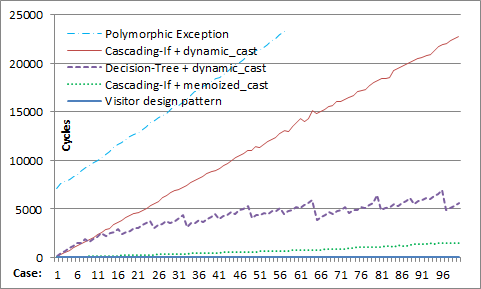
\includegraphics[width=0.47\textwidth]{DCast-vs-Visitors1.png}
  \caption{Time to uncover type in the $i^{th}$ case clause}
  \label{fig:DCastVis}
\end{figure}

When the class hiearchy is not flat and has several levels, the above 
cascading-if can be replaced with a decision tree that tests base classes first 
and thus eliminates many of the derived classes from consideration. This 
approach is used by Emir to deal with type patterns in Scala
\cite[\textsection 4.2]{EmirThesis}. The intent is to replace a sequence of 
independent dynamic casts between classes that are far from each other in the 
hierarchy with nested dynamic casts between classes that are closer to each 
other. Another advantage is possiblity to fail early: if the type of the object 
in quesion does not match any of the clauses, we will not have to try all the 
cases. Flat hierarchy, which will likely be formed by the leafs in an even 
multi-level hiearrchy, will not be able to benefit from this optimization and 
will effectively degrade to the above cascading-if. Nevertheless, when 
applicable the optimization can be very useful and its benefits can be seen in
Figure~\ref{fig:DCastVis} under ``Decision tree dynamic\_cast''. The class 
hierarchy for this timing experiment was forming a perfect binary tree with 
classes with number 2*N and 2*N+1 derived from a class with number N.

While looking for alternatives to visitor design pattern it became clear that 
any open solution that will have a non-constant dispatching overhead will 
have a poor chance of being adopted. Switching on sequentially allocated tags
was one of the few techniques that could achieve constant overhead, even smaller 
than that of visitors, but it had problems of its own that were making it not
suitable. To better understand the problem let us look at some existing 
solutions to type switching that we found to be used in practice.

%From our experience on this project we have noticed that we can only compete 
%with visitors when switch statements are implemented with a jump table. As soon 
%as compiler was putting even a single branch into the decision tree of cases, 
%the performance was degraded significantly. From this perspective we do not 
%regard solutions based on decision trees as efficient, since they do not let us 
%compete compete with the visitors solution.

The simple scheme of assigning a unique tag per variant (instantiatable class 
here) will not pass the first question because the tags of base and derived 
classes will have to be different if the base class can be instantiated on its 
own. When the base class is used as an interface only and is never instantiated, 
the already mentioned partitioning of tags of derived classes could have been 
used, but that again will assume knowledge of all the classes and thus fail 
extensibility through DLLs.

Often time tags are chosen not arbitrarily, but to reflect the subtyping 
relation of the underlain hierarchy. An example of such scheme would be having a 
certain bit in the tag set for all the classes derived from a given base class.  
Switching on base classes then involves a call to some function $f$ that 
converts derived class' tag into a base class' tag. Unfortunately this solution 
creates more problems then it solves. 

First of all the solution will not be able 
to recognize an exceptional case where most of the derived classes should be 
handled as base class, while few should be handled specifically. Applying 
function $f$ puts several different types into an equivalence class with their 
base type, making them indistinguishable from each other. 

Secondly, the assumed 
structure of tags is likely to make the set of tags sparce, effectively forcing 
compiler to use a decision tree instead of jump table to implement the switch.
Even though conditional jump is reported to be faster than indirect jump on many 
computer architectures~\cite[\textsection 4]{garrigue-98}, this did not seem to 
be the case in our experiments. Spliting of a jump table into two with a 
condition, that was sometimes happening because of our case label allocation 
scheme, was resulting in a noticable degradation of performance in comparison to 
a single jump table.

The assumed structure of tags can also significantly decrease the amount of 
classes a given allocation scheme can handle. Allocation scheme used by Gibbs et 
al to implement fast dynamic casting employs divisibility of numbers to 
represent inheritance relation\cite{FastDynCast}. A 32-bit integer is estimated 
to be able to represent 7 levels of a class hierarchy that forms a binary tree 
(255 classes), 6 levels of a similar ternary tree hierarchy (1093 classes) or 
just one level of a hierarchy with 9 base classes -- multiple inheritance is the 
worst case scenario of the scheme that quickly drains it of allocation 
possibilities. It is interesting to note that the above scheme can be easily adopted to implemented type switching with decision trees, it is not easily adoptable for type switching: 
in order to obtain tags of base classes we will have to decompose the derived 
tag into primes

To the best of our knowledge we are unaware of any tag allocation scheme capable 
of dealing with all of the above isues that can be incorporated efficiently into  
a switch statement to form a type switch.

Our approach can be used together with backtracking or decision tree approaches. 
Instead of a linear search our current macros generate simply to because we 
depend on the syntacti order of definitions in library setting, the compiler may 
generate either a decision tree or backtracking automata to find the applicable 
type. After that the compiler would just cache the jump target inside the 
function.

The approach can also be used to optimize handling of polymorphic variants in 
OCaml when implemented as proposed by Garrigue\cite{garrigue-98}. The tag values 
compiler generates for each of the variants can be seen as vtbl pointer value 
and a similar memoization device can be embedded into a decision tree.

%%%%%%%%%%%%%%%%%%%%%%%%%%%%%%%%%%%%%%5555

\noindent
We chose to give it a first-fit semantics in our library as it was resembling 
pattern matching facilities of other languages and was the most intuitive. The 
following code can be generated to implement it:

\begin{lstlisting}
if (D1* derived = dynamic_cast<D1*>(base)) { s1; } else
if (D2* derived = dynamic_cast<D2*>(base)) { s2; } else
...
if (Dn* derived = dynamic_cast<Dn*>(base)) { sn; }
\end{lstlisting}

\noindent
Note that leaving \code{else} out will effectively turn it into an all-fit 
statement with enabled statements executed in lexicographical order.

The above code is easy to understand but is extremely inefficient as for an 
object of dynamic type $D_i$ we will have to perform $i-1$ dynamic casts that 
fail first. The diagram below compares the times spent by visitors and the above 
type switch statement to uncover the $i^{th}$ case. We postpone the discussion 
of \code{memoized_cast} until section \textsection\ref{}, here we would only 
like to notice that even though faster than the actual dynamic cast it also bears 
a linear coefficient, not present in visitors.

\subsection{Memoization Device}

Let's look at slightly more general problem. Consider a generalization of switch 
statement that takes predicates on a selector as its clauses and executes the 
first statement $s_i$ whose predicate got enabled:

\begin{lstlisting}
switch (x)
{
    case P1(x): s1;
    ...
    case Pn(x): sn;
}
\end{lstlisting}

\noindent
Assuming that predicates depend only on $x$ and nothing else we can be sure that
the next time we come to such switch with the same value, the same predicate 
will become enabled first. Thus we would like to avoid evaluating predicates and 
jump straight to the statement it guards. In a way we would like the switch to 
memoize which case becomes enabled for a given value of $x$. 

Inspired by Duff's Device\cite{Duff} we devised a construct that we call 
\emph{Memoization Device} that does just that.

\begin{lstlisting}
typedef decltype(x) T;
static std::unordered_map<T,int> memory;

switch (int& target = memory[x])
{
default:
    if (P1(x)) { target = 1;
case 1:
        s1;
    } else 
    if (P2(x)) { target = 2;
case 2:
        s2;
    } else
 ...
    if (Pn(x)) { target = N;
case N:
        sN;
    } else       target = N+1;
case N+1:
}
\end{lstlisting}

Upon first entry into such a function we will allocate a static map associating 
values we are memoizing to cases labels. A value $x$ that is not yet in the map 
will result in an new entry allocated with its data (of type int) being default 
initialized to 0. switch on a value 0 will take us to default statement, which 
will iniate going over cascading-if in a normal way. 

Assuming that predicate Pi(x) returns true, we will store i as a target 
associated with $x$ so that the next time we are called with the value $x$ we 
can jump directly to label i. If none of the predicates returned true, we will 
record it by setting target to N+1, so that the next time we can jump directly 
to the end of the switch on such $x$. 

In certain cases we might want to be able to preserve the fall-through behavior 
of a switch and be able to evaluate all statements, whose predicates are true. 
In such case we might still prefer to skip the initial predicates returning 
false, starting from the first successful one. This can easily be achieved by 
removing all else statements, making all if-statements independent, but wrapping 
all assignments to target with condition, to make sure only the first 
successfult predicate executes it:

\begin{lstlisting}
 ...
    if (Pi(x)) { 
        if (target == 0)
            target = i;
case i:
        si;
    }
\end{lstlisting}

Note that the protocol that has to be maintained by this structure does not 
depend on the actual value of case labels. The only thing we rely on here is 
that they are all different and that there is a predefined default value, not 
equal to any of them as well. In fact, the default clause we used here could 
have been replaced with case clause with that predefined value. From experience,
however, we have noticed that keeping the default clause results in a faster 
code. A more important performance consideration is to keep the values close to
each other. Not following this rule might result in compiler choosing decision 
tree over a jump table implementation, which will significantly degrade 
performance.

The main advantage of such a device is that it does not impose any restriction 
on the type of a selector. It can easily support multiple scrutinee by turning 
$x$ into a tuple. One has to be careful however to make sure his predicates do 
not involve global state. Another advantage is that conditions and statements 
do not have to be repeated several times textually, which lets us turn the 
boilerplate code of maintaining memoization logic into macros.

The main disadvantage of such solution is of course the size of table that grows 
proportionally to the amount of different values coming through the function. We 
will see, however, that often times the values can be grouped into equivalence 
classes, such that values in the same class do not change the predicate. The map 
can then associate an equivalence class with target.

\subsection{Virtual Table Pointers}

Before we discuss our solution we would like to talk about certain properties of 
the C++ run-time system that we rely on. Strictly speaking C++ standard does not 
require implementations to use any given technique, however interoperability 
requirements have forced compiler vendors to design a set of rules called 
Application Binary Interface (ABI)\cite{C++ABI}. Most of the C++ compilers today 
follow these rules, with notable exception of Microsoft Visual C++. We show that 
the technique presented here will work with any C++ compiler that follows the 
C++ ABI.

Besides traditional single inheritance on classes, C++ supports 
multiple-inheritance of two kinds: repeated and virtual. Under repeated 
inheritance given derived class may inherit certain base class in several ways. 
Objects of such class will have several subobjects of that base class. Under 
virtual inheritance there will only be one shared subobject, accessible through 
different inheritance paths.

\begin{figure}[tbp]
  \centering
    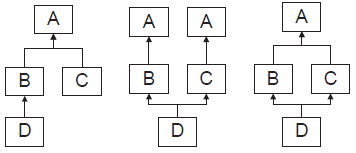
\includegraphics[width=0.47\textwidth]{Hierarchies.png}
  \caption{Single inheritance, repeated multiple inheritance and virtual multiple inheritance}
  \label{fig:hierarchy}
\end{figure}

\noindent
Note that the above picture portrais subobject relatedion, not the inheritance.

The notion of subobject has been formalized before\cite{RF95,WNST06,RDL11}.
We follow here the presentation of Ramamanandro et al\cite{RDL11}.

A base class subobject of a given complete object is represented by a pair 
$\sigma = \langle h,l\rangle$ with $h \in \{Repeated,Shared\}$ representing the 
kind of inheritance (single inheritance is repeated with one base class) and $l$ 
representing the path in non-virtual inheritance graph.

A predicated $C\leftY\sigma\rightY A$ they introduce means that $\sigma$ 
designates a base class subobject of class $C$, with subobject's static type 
being $A$. (Give recursive definition and more explanations from Layout paper).

A class that declares or inherits a virtual function is called a 
\emph{polymorphic class}\cite[\textsection 10.3]{C++0x}. C++ ABI in turn defines 
\emph{dynamic class} to be a class requiring a \emph{virtual table pointer} 
(because it or its bases have one or more virtual member functions or virtual 
base classes). A polymorphic class is thus a dynamic class by definition.

A \emph{primary base class} for a dynamic class is the unique base class (if any) 
with which it shares the virtual table pointer at offset 0. The data layout 
procedure for non-POD types described in \textsection2.4 of C++ ABI 
requires dynamic classes either to allocate vtable pointer at offset 0 or share 
the virtual table pointer from its primary base class, which is by definition at 
offset 0. For our purpose this means that we can rely on virtual table pointer 
always be present at offset 0 for dynamic classes.

C++ standard requires an argument of \code{dynamic_cast} to be a pointer to or 
an lvalue of a polymorphic type when performing \emph{downcast} -- a cast from 
base to derived.\cite[\textsection 5.2.7-6]{C++0x}. And since polymorphic type 
is dynamic type and dynamic types always have virtual table pointer at offset 0, 
we can safely extract such a pointer from an expression that was intended to be 
an argument of a \code{dynamic_cast} (e.g. from a type switch).

A dynamic class, accordingly to ABI, has an associated table (often several 
instances, but not one per object) called virtual table (or vtable). 
\emph{Virtual table} is a table of information used to dispatch virtual 
functions, access virtual base class subobjects, and to access information for 
runtime type identification (RTTI). \emph{Virtual table pointer} is a member of 
object's layout pointing to a virtual table. Because of repeated inheritance an 
object of given type may have several virtual table pointers in it. Each such 
pointer corresponds to one of the polymorphic base classes. 

Similarly, each class that has virtual member functions or virtual bases has an 
associated set of virtual tables. There may be multiple virtual tables for a 
particular class, if it is used as a base class for other classes. However, the 
virtual table pointers within all the objects (instances) of a particular 
most-derived class point to the same set of virtual tables.

The exact content of the virtual table is not important for this discussion. We 
would like to point out a few fields in it that we will refer to later.

\begin{itemize}
\item The \emph{typeinfo pointer} points to the typeinfo object used for RTTI. 
      It is always present.  
\item The \emph{offset to top} holds the displacement to the top of the object 
      from the location within the object of the virtual table pointer that 
      addresses this virtual table, as a \code{ptrdiff_t}. It is always present.
\item \emph{Virtual Base (vbase) offsets} are used to access the virtual bases 
      of an object. Such an entry is added to the derived class object address 
      (i.e. the address of its virtual table pointer) to get the address of a 
      virtual base class subobject. Such an entry is required for each virtual 
      base class.
\end{itemize}

\noindent
Given a virtual table pointer \code{vtbl}, we will refer to these fields as 
\code{rtti(vtbl)}, \code{off2top(vtbl)} and \code{vbase(vtbl)} respectively. 
Given an object $a$ of static type $A$ that has $k$ virtual table pointers in 
it, we will use the same notion we use for regular fields to access them: 
$a.vtbl_i$. We also assume presence of function $offset(\sigma)$ that defines 
the offset of the base class identified by the end of the path $\sigma$ within a 
class identified by its first element.

We would like to point out that during construction and deconstruction of an 
object, a value of a given virtual table pointer may change. In particular that 
value will reflect the dynamic type of the object to be the type of the fully 
constructed part only. This will not affect our reasoning, howver, as during 
such transition we treat the object to be the type of its fully constructed 
base only. Once the complete object is fully constructed, the value of the 
virtual table pointer will remain the same for the lifetime of the object.

%general virtual table pointer will not be pointing to the beginning of actual 
%virtual table, but to an \emph{address point of the virtual table}. The virtual 
%table will therefore contain components at either positive or negative offsets 
%from its address point.

\begin{theorem}
In an object layout that adheres to C++ ABI, virtual table pointers of two 
objects of the same static type are equivalent if and only if they have the same 
inheritance path in the same most-derived type.
%belong to the same subobject of 
\begin{eqnarray*}
    \forall a_1, a_2 : A\ |\ a_1\in C_1\leftY\sigma_1\rightY A \wedge a_2\in C_2\leftY\sigma_2\rightY A \\
    a_1.vtbl_i = a_2.vtbl_i \iff C_1 = C_2 \wedge \sigma_1 = \sigma_2
\end{eqnarray*}
\end{theorem}
\begin{proof}
Let's assume first $a_1.vtbl_i = a_2.vtbl_i$ but $C_1 \neq C_2$. In this case we 
have \code{rtti}$(a_1.vtbl_i) = $\code{rtti}$(a_2.vtbl_i)$. By definition 
\code{rtti}$(a_1.vtbl_i) = C_1$ while \code{rtti}$(a_2.vtbl_i) = C_2$, which 
contradicts that $C_1 \neq C_2$. Thus $C_1 = C_2 = C$.

Let's assume now that $a_1.vtbl_i = a_2.vtbl_i$ but $\sigma_1 \neq \sigma_2$. 
Let $\sigma_i=\langle h_i,l_i\rangle,i=1,2$ 

If $h_1 \neq h_2$ then one of them refers to virtual base while the other to 
repeated. Assuming $h_1$ refers to virtual path, \code{vbase}$(a_1.vtbl_i)$ has 
to be defined inside the vtable accordingly to ABI, while 
\code{vbase}$(a_2.vtbl_i)$ -- should not. This would contradict again that both 
$vtbl_i$ refer the same virtual table.

We have thus $h_1 = h_2 = h$. If $h = Shared$ than there is only one path to 
such $A$ in $C$, which would contradict $\sigma_1 \neq \sigma_2$. 
If $h = Repeated$ then we must have that $l_1 \neq l_2$. In this case let $k$ be 
the first position in which they differ: 
$l_1^j=l_2^j \forall j<k \wedge l_1^k\neq l_2^k$. Since our class $A$ is a base 
class for classes $l_1^k$ and $l_2^k$, both of which are in turn base classes of 
$C$, object identity requirement of C++ require that the relevant subobjects of 
type $A$ have different offsets within class $C$: 
$offset(\sigma_1)\neq offset(\sigma_2)$ However 
$offset(\sigma_1)=$\code{off2top}$(a_1.vtbl_i)=$\code{off2top}$(a_2.vtbl_i)=offset(\sigma_2)$ 
since $a_1.vtbl_i = a_2.vtbl_i$, which contradicts that offsets are different.

Conjecture in the other direction is trivial since subobjects on the same 
inheritance path in different instances will get initialized with the same 
vtable pointers.
\end{proof}

\begin{corollary}
Results of \code{dynamic_cast} can be reapplied to a different instance from the same subobject.
$\forall a_1, a_2 : A\ |\ a_1.vtbl_i = a_2.vtbl_i \Rightarrow$
\code{dynamic_cast<B>}$(a_1).vtbl_j = $\code{dynamic_cast<B>}$(a_2).vtbl_j \vee$ \\
\code{dynamic_cast<B>}$(a_1)$ throws $\wedge$ \code{dynamic_cast<B>}$(a_2)$ 
throws.
\end{corollary}

\subsection{VTable Memoization}

Since the results of dynamic cast can be reapplied on objects with the same 
virtual table pointer, we can now apply memoization device to polymorphic 
objects grouped by their virtual table pointer. The head of the switch requires 
few extra definitions:

\begin{lstlisting}
typedef pair<ptrdiff_t,size_t> type_switch_info;
static std::unordered_map<intptr_t, type_switch_info> memory;
intptr_t          vtbl = *reinterpret_cast<const intptr_t*>(p);
type_switch_info& info = memory[vtbl];
const void*       tptr; 
\end{lstlisting}

We use the virtual table pointer extracted from a polymorphic object pointed to 
by \code{p} as a key for association. The value stored along the key in 
association now keeps both: the target for the switch as well as a memoized 
offset for dynamic cast. The snippet corresponding to the $i^{th}$ case now 
looks as following:

\begin{lstlisting}
    if (tptr = dynamic_cast<const Di*>(p))
    {
        if (info.second == 0)
        {
            info.first  = intptr_t(tptr)-intptr_t(p);
            info.second = 42;
        }
case 42:
        auto matched = adjust_ptr<Di>(p,info.first); 
        si;
    }
\end{lstlisting}

\noindent
The main condition remains the same. We keep check for the first initialization 
because we allow the fall-through semantics here, letting user break fromt the 
switch when needed. Upon first entry we compute the offset that the dynamic cast 
performed and save it together with targed associated to the virtual table 
pointer. On the next iteration we will jump directly to the case label and 
restore the invariant of \code{matched} being a properly casted reference to the 
derived object.

\begin{figure}[htbp]
  \centering
    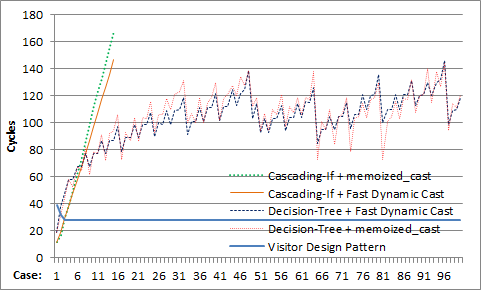
\includegraphics[width=0.47\textwidth]{DCast-vs-Visitors2.png}
  \caption{Time to uncover i\textsuperscript{th} case. X-axis - case i; Y-axis - cycles per iteration}
  \label{fig:DCastVis2}
\end{figure}

The net effect of this optimization can be seen in Figure~\ref{fig:DCastVis2}. 
We can see that the time does not increase with the position of the case we are 
handling. The spikes represent activities on computer during measurement and are 
present in both measurements. The type switch is still about 50\% slower, and 
making it even faster is discussed in the next subsection.

\subsection{Structure of Virtual Table Pointers}

\subsection{Redundancy Checking}
\label{sec:redun}

Our library lets the compiler check the case clauses for redundancy by defining 
a macro that triggers generation of additional syntactic structure. The 
structure effectively generates a try-catch statement based on the target types 
of case clauses, which forces the compiler to give warning when more general 
catch handler preceeds more specific one e.g.:

\begin{lstlisting}
filename.cpp(55): warning C4286: 'ipr::Decl*' : is caught by 
                  base class ('ipr::Stmt*') on line 42
\end{lstlisting}

\noindent
Note that message contains both: a line number of the redundant case (55) and 
the line number of the case it is made redundant with (42).

\subsection{Open Case}

To put further explanations into perspective as well understand the problem 
better we present some timing measurements of straightforward, but rather naive 
implementation of a match statement outlined in \textsection\ref{sec:semms}.

\subsection{Closed Case}

%[FROM ABI: 2.4 I 2.c] If C has no primary base class, allocate the virtual 
%table pointer for C at offset zero, and set sizeof(C), align(C), and dsize(C) to 
%the appropriate values for a pointer (all 8 bytes for Itanium 64-bit ABI).

%[FROM ABI: 2.5.2]
%The offset to top holds the displacement to the top of the object from the 
%location within the object of the virtual table pointer that addresses this 
%virtual table, as a  ptrdiff_t. It is always present. The offset provides a way 
%to find the top of the object from any base subobject with a virtual table 
%pointer. This is necessary for dynamic_cast<void*> in particular.

%The typeinfo pointer points to the typeinfo object used for RTTI. It is always 
%present. All entries in each of the virtual tables for a given class must point 
%to the same typeinfo object. A correct implementation of typeinfo equality is to 
%check pointer equality, except for pointers (directly or indirectly) to 
%incomplete types. The typeinfo pointer is a valid pointer for polymorphic 
%classes, i.e. those with virtual functions, and is zero for non-polymorphic 
%classes.



\section{Evaluation} %%%%%%%%%%%%%%%%%%%%%%%%%%%%%%%%%%%%%%%%%%%%%%%%%%%%%%%%%%%
\label{sec:eval}

\begin{figure*}
\begin{tabular}{@{}c@{ }l||@{ }r@{}@{ }r@{}@{ }r@{}|@{ }r@{}@{ }r@{}@{ }r@{}||@{ }r@{}@{ }r@{}@{ }r@{}|@{ }r@{}@{ }r@{}@{ }r@{}||@{ }r@{}@{ }r@{}@{ }r@{}|@{ }r@{}@{ }r@{}@{ }r@{}}
\hline % -----------------------------------------------------------------------------------------------------------------------------------------
\hline % -----------------------------------------------------------------------------------------------------------------------------------------
 &            & \multicolumn{6}{c||}{G++/32}                  & \multicolumn{6}{c||}{MS Visual C++/32}        & \multicolumn{6}{c}{MS Visual C++/64}           \\
\hline % -----------------------------------------------------------------------------------------------------------------------------------------
 & Syntax     & \multicolumn{3}{c|}{Unified} & \multicolumn{3}{c||}{Specialized} & \multicolumn{3}{c|}{Unified} & \multicolumn{3}{c||}{Specialized} & \multicolumn{3}{c|}{Unified} & \multicolumn{3}{c}{Specialized} \\
\hline % -----------------------------------------------------------------------------------------------------------------------------------------
 & Encoding   & \Opn  & \Cls  & \Unn  & \Opn  & \Cls  & \Unn  & \Opn  & \Cls  & \Unn  & \Opn  & \Cls  & \Unn  & \Opn  & \Cls  & \Unn  & \Opn  & \Cls  & \Unn   \\
\hline % -----------------------------------------------------------------------------------------------------------------------------------------
\hline % -----------------------------------------------------------------------------------------------------------------------------------------
 & Repetitive &\gwNGPp&\gwNGKp&\gwNGUp&\gwNSPp&\gwNSKp&\gwNSUp&\vwNGPp&\vwNGKp&\vwNGUp&\vwNSPp&\vwNSKp&\vwNSUp&\vxNGPp&\vxNGKp&\vxNGUp&\vxNSPp&\vxNSKp&\vxNSUp \\
 & Sequential &\gwNGPq&\gwNGKq&\gwNGUq&\gwNSPq&\gwNSKq&\gwNSUq&\vwNGPq&\vwNGKq&\vwNGUq&\vwNSPq&\vwNSKq&\vwNSUq&\vxNGPq&\vxNGKq&\vxNGUq&\vxNSPq&\vxNSKq&\vxNSUq \\
 & Random     &\gwNGPn&\gwNGKn&\gwNGUn&\gwNSPn&\gwNSKn&\gwNSUn&\vwNGPn&\vwNGKn&\vwNGUn&\vwNSPn&\vwNSKn&\vwNSUn&\vxNGPn&\vxNGKn&\vxNGUn&\vxNSPn&\vxNSKn&\vxNSUn \\
\hline % ------------------------------------------------------------------------------------------------------------------------------------------
\multirow{3}{*}{\begin{sideways}{\tiny Forward}\end{sideways}}
 & Repetitive &\gwYGPp&\gwYGKp&\gwYGUp&\gwYSPp&\gwYSKp&\gwYSUp&\vwYGPp&\vwYGKp&\vwYGUp&\vwYSPp&\vwYSKp&\vwYSUp&\vxYGPp&\vxYGKp&\vxYGUp&\vxYSPp&\vxYSKp&\vxYSUp \\
 & Sequential &\gwYGPq&\gwYGKq&\gwYGUq&\gwYSPq&\gwYSKq&\gwYSUq&\vwYGPq&\vwYGKq&\vwYGUq&\vwYSPq&\vwYSKq&\vwYSUq&\vxYGPq&\vxYGKq&\vxYGUq&\vxYSPq&\vxYSKq&\vxYSUq \\
 & Random     &\gwYGPn&\gwYGKn&\gwYGUn&\gwYSPn&\gwYSKn&\gwYSUn&\vwYGPn&\vwYGKn&\vwYGUn&\vwYSPn&\vwYSKn&\vwYSUn&\vxYGPn&\vxYGKn&\vxYGUn&\vxYSPn&\vxYSKn&\vxYSUn \\
\hline % -----------------------------------------------------------------------------------------------------------------------------------------
\hline % -----------------------------------------------------------------------------------------------------------------------------------------
 &            & \multicolumn{6}{c||}{G++/32}                  & \multicolumn{6}{c||}{MS Visual C++/32 with PGO} & \multicolumn{6}{c}{MS Visual C++/64 with PGO} \\
\hline % -----------------------------------------------------------------------------------------------------------------------------------------
 & Syntax     & \multicolumn{3}{c|}{Unified} & \multicolumn{3}{c||}{Specialized} & \multicolumn{3}{c|}{Unified} & \multicolumn{3}{c||}{Specialized} & \multicolumn{3}{c|}{Unified} & \multicolumn{3}{c}{Specialized} \\
\hline % -----------------------------------------------------------------------------------------------------------------------------------------
 & Encoding   & \Opn  & \Cls  & \Unn  & \Opn  & \Cls  & \Unn  & \Opn  & \Cls  & \Unn  & \Opn  & \Cls  & \Unn  & \Opn  & \Cls  & \Unn  & \Opn  & \Cls  & \Unn   \\
\hline % -----------------------------------------------------------------------------------------------------------------------------------------
\hline % -----------------------------------------------------------------------------------------------------------------------------------------
 & Repetitive &\GwNGPp&\GwNGKp&\GwNGUp&\GwNSPp&\GwNSKp&\GwNSUp&\VwNGPp&\VwNGKp&\VwNGUp&\VwNSPp&\VwNSKp&\VwNSUp&\VxNGPp&\VxNGKp&\VxNGUp&\VxNSPp&\VxNSKp&\VxNSUp \\
 & Sequential &\GwNGPq&\GwNGKq&\GwNGUq&\GwNSPq&\GwNSKq&\GwNSUq&\VwNGPq&\VwNGKq&\VwNGUq&\VwNSPq&\VwNSKq&\VwNSUq&\VxNGPq&\VxNGKq&\VxNGUq&\VxNSPq&\VxNSKq&\VxNSUq \\
 & Random     &\GwNGPn&\GwNGKn&\GwNGUn&\GwNSPn&\GwNSKn&\GwNSUn&\VwNGPn&\VwNGKn&\VwNGUn&\VwNSPn&\VwNSKn&\VwNSUn&\VxNGPn&\VxNGKn&\VxNGUn&\VxNSPn&\VxNSKn&\VxNSUn \\
\hline % ------------------------------------------------------------------------------------------------------------------------------------------
\multirow{3}{*}{\begin{sideways}{\tiny Forward}\end{sideways}}
 & Repetitive &\GwYGPp&\GwYGKp&\GwYGUp&\GwYSPp&\GwYSKp&\GwYSUp&\VwYGPp&\VwYGKp&\VwYGUp&\VwYSPp&\VwYSKp&\VwYSUp&\VxYGPp&\VxYGKp&\VxYGUp&\VxYSPp&\VxYSKp&\VxYSUp \\
 & Sequential &\GwYGPq&\GwYGKq&\GwYGUq&\GwYSPq&\GwYSKq&\GwYSUq&\VwYGPq&\VwYGKq&\VwYGUq&\VwYSPq&\VwYSKq&\VwYSUq&\VxYGPq&\VxYGKq&\VxYGUq&\VxYSPq&\VxYSKq&\VxYSUq \\
 & Random     &\GwYGPn&\GwYGKn&\GwYGUn&\GwYSPn&\GwYSKn&\GwYSUn&\VwYGPn&\VwYGKn&\VwYGUn&\VwYSPn&\VwYSKn&\VwYSUn&\VxYGPn&\VxYGKn&\VxYGUn&\VxYSPn&\VxYSKn&\VxYSUn \\
\hline % -----------------------------------------------------------------------------------------------------------------------------------------
\end{tabular}
\caption{Relative performance of our pattern matching versus visitors. Numbers 
like \f{42} in bold font indicate that our pattern matching is faster than 
visitors by corresponding percentage. Numbers like \s{42} in italics font 
indicate that our solution is slower than visitors (i.e. visitors is faster than 
our solution) by corresponding percentage.}
\label{relperf}
\end{figure*}

In this section we evaluate the performance of our solution in comparison to its 
de facto contender -- visitor design pattern. We also compare performance of 
some typical uses cases expressed with our solution and OCaml.

Our evaluation methodology consists of several benchmarks that we believe 
represent various possible uses of objects analized with either visitors or 
pattern matching.

\begin{itemize}
\item Repetitive
\item Sequential
\item Random
\item Forwarding
\end{itemize}

\emph{Repetitive} benchmark performs multiple calls on one and the same object. 
This scenario often happens in object-oriented setting because of encapsulation 
where multiple callees effectively reevaluate the same method in order not to 
pass additional context around. Most of the data related to such call is usually 
present in cache.

\emph{Sequential} benchmark effectively uses object of each derived type only 
once and then moves on to an object of a different type. The cache is typically 
reused the least in this scenario. The scenario is typical of lookup tables, 
where each entry is implemented with a different derived class.

\emph{Random} benchmark is the most representative as it randomly makes calls on 
random objects, which will probably be the most common usage scenario in the 
real world.

\emph{Forwarding} benchmark is not a benchmark on its own, but rather a 
combinator that can be applied to any of the above scenarios. It refers to the 
common technique used by visitors where for class hierarchies with multiple 
levels of inheritance the \code{visit} method of a derived class will provide a 
default implementation of forwarding to its immediate base class, who in turn 
may forward it to its base class etc. This approach is used in Pivot, whose AST 
hierarchy consists of 154 node kinds, of which only 5 must be handled, while the 
rest will forward to them when visit for them was not overriden.

These benchmarks were executed in the following configurations:

\begin{itemize}
\item Sony VAIO\textsuperscript{\textregistered} laptop with Intel\textsuperscript{\textregistered} Core\texttrademark i5 460M 
      Processor at 2.53 GHz equipped with 6GB of RAM running Windows 7 
      Professional
      \begin{itemize}
      \item G++ 4.5.2 under MinGW executed with -O2 and producing x86 binary
      \item MS Visual C++ 2010 Professional
            \begin{itemize}
            \item x86 binary
            \item x64 binary
            \item x86 binary with Profile Guided Optimizations
            \item x64 binary with Profile Guided Optimizations
            \end{itemize}
      \end{itemize}
\end{itemize}

Each benchmark under each configuration were tested with either \emph{unified} 
or \emph{specialized} syntax. Each syntax was used to run tests on \emph{Open} 
(generalization of \emph{polymorphic base class} encoding), \emph{Tag} 
(generalization of \emph{tag class} encoding) and \emph{Union} (same as 
\emph{discriminated union} encoding). Specialized syntax avoids generating 
unnecessary syntactic structure used to unify syntax and thus produces faster 
code. We include it in results as compiler implementation of pattern matching 
will be able to distinguish each case and thus generate only the required 
structure.

We include results of optimizing code created with Visual C++ by using profile 
guided optimizations as currently Visual C++ does not have means for branch 
hinting, which are supported by G++ and proven to be very effective in few 
cruicial places. Profile guided optimization in Visual C++ lets compiler find 
out experimentally what we would have otherwise hinted, even though this 
includes other optimizations as well.

We compare performance of our solution relatively to performance of visitors in 
Figure~\ref{relperf}. The values are given as percentage of performance increase 
against the slower technique. Numbers in bold represent cases where our pattern 
matching was faster than visitors and indicate corresponding percentage. Numbers 
in italics indicate cases where visitors were faster (and thus we were slower) 
by given percentage.

From the numbers given we can see that pattern matching wins by a good margin in 
the presense of at least one level of forwarding on visitors. Using pattern 
matching on closed hierarchies is a definite winner that providing the same 
unified syntax. Use of specialized syntax always results in a faster pattern 
matching code by avoiding unification overhead.

The code for x64 is only slower relatively: the actul time spent for both 
visitors and pattern matching was smaller than that for x86, but it was much 
smaller for visitors than pattern matching, which resulted in worse relative 
performance.

\subsection{Qualitative Comparison}

For this experiment we have reimplemented a visitor based C++ pretty printer for 
Pivot's IPR using our pattern matching library. Most of the rewrite was 
performed by sed-like replaces that converted visit methods into respective 
case-clauses. In several cases we had to manually reorder case-clauses to avoid 
redundancy as visit-methods for base classes were typically coming before the 
same for derived, while for pattern matching we needed them to come after. 
Redundancy checking support in the library discussed in \textsection\ref{sec:redun}
was invaluable in finding out all such cases.

During this refactoring we have made several simplifications that became obvious 
in pattern-matching code, but were not in visitors code because of control 
inversion. Simplifications that were applicable to visitors code were eventually 
integrated into visitors code as well to make sure we do not compare 
algorithmically different code. In any case we were making sure that both 
approaches regardless of simplifications were producing byte-to-byte the same 
output as the original pretty printer we started from.

The size of executable for pattern matching approach was smaller than that for 
visitors. So was also the source code. We extracted from both sources the 
functionality that was common to them and placed it in a separate translation 
unit to make sure it does not participate in the comparison. We kept all the 
comments however that were eqaully applicable to code in either approach.

Note that the visitors involved in the pretty printer above did not use 
forwarding: since all the C++ constructs were handled by the printer, every 
visit-method was overriden from those statically possible based on the static 
type of the argument.

%Listing parameter for a case clause always causes access to member. Best hope is 
%that compiler will eliminate it if it is not needed. At the moment we do not 
%have means to detect empty macro arguments or \_.

To be continued...

In general from our rewriting experience we will not recommend rewriting 
existing visitor code with pattern matching for the simple reason that pattern 
matching code will likely follow the structure already set by the visitors. 
Pattern matching was most effective when writing new code, where we could design 
the structure of the code having the pattern matching facility in our toolbox.

\section{Discussion} %%%%%%%%%%%%%%%%%%%%%%%%%%%%%%%%%%%%%%%%%%%%%%%%%%%%%%%%%%%
\label{sec:dsc}

We considered using smaller types for storing line numbers based on our 
observation that we have not found many C++ source files that had more than 65535 
lines. This was saving us space for hash tables but resulted in worse 
performance due to access of smaller words from memory.

We also looked into storing differences between switch's head line number and 
case's line number, following the observation that very occasionally we saw more 
than 256 cases in a pattern-matching switch. This also degraded performance so 
we did not use it.

We would like to note that in presence of deeper hierarchy, visitors often 
implement members by forwarding call to their base, which may incur additional 
overhead.

\section{Related Work} %%%%%%%%%%%%%%%%%%%%%%%%%%%%%%%%%%%%%%%%%%%%%%%%%%%%%%%%%
\label{sec:rw}

Spuler compares a number of techniques in implementing switch 
statements\cite{Spuler94}.

A good survey of work on general pattern matching can be found in in a term 
project paper by Miller\cite{Miller10}.

Great overview of pattern matching in Scala compared to several other languages 
is presented in\cite{ScalaPM}.

Prop was an attempt to add pattern matching together with algebraic data types 
and other functional features into C++\cite{Prop96}.

JMatch was a similar incentive to add pattern matching to Java.

Sankel provides a good educational overview of how algebraic data types can be 
implemented in C++\cite{SankelFP10,Sankel10}. 

Emir's PhD thesis provides an extensive analysis of pattern matching in the 
context of object-oriented languages\cite{EmirThesis}.

Cook et al used expression templates to implement a query language to Pivot's 
IPR\cite{iql04}. The principal difference of their work from this work is that 
authors were essentially creating a pattern matcher for a given class hierarchy 
and thus could take the semantics of the entities represented by classes in the 
hierarchy into account. Our approach is parametrized over class hierarchy and 
thus provides a rather lower level pattern-matching functionality that lets one 
simplify work with that hierarchy.  One can think of it as a generalized 
dynamic\_cast.

In his dissertation, Pirkelbauer provides a different pattern matcher against 
Pivot's IPR\cite{PirkelbauerThesis}.

Veldhuizen discovered a very powerful technique called Expression 
templates\cite{Veldhuizen95expressiontemplates}.

Other languages that use pattern matching include: ...

Dos Reis et al compares functional and imperative approaches to generic 
programming and discusses the role of pattern matching in expressing generic 
algorithms in the functional approach\cite{dos_reis:05:what_is_gp}. They also 
demonstrate with an elegant example the amount of boilerplate code necessary to 
write in C++ in order to describe a sum-functor.k

Boost::proto is a library for creating DSL using expression templates.

TOM is a pattern matching compiler that adds pattern-matching facilities to 
imperative languages such as C, Java, or Eiffel.\cite{Moreau:2003}

%[From Extensible Algebraic Datatypes with Defaults]
%The traditional object-oriented and functional approaches
%both make extensions in one dimension easy, but extensions
%in the other dimension very hard. In the object-oriented approach,
%data is modelled by a set of classes, sharing a common
%interface. For the lambda term example, there would
%be an interface or abstract class Term specifying the eval
%method with subclasses Lambda, Apply and Variable. Each
%subclass defines its own implementation of eval. W hereas
%extending the datatype with new variants is simply done by
%creating new classes, adding new operations involves modifications
%of the abstract base class.
%On the other hand, in the functional approach, the variants
%of a datatype are typically implemented as an algebraic
%type. Here, defining new operations is easy. One just writes
%a new function which matches against the data variants.
%But since ordinary algebraic datatypes cannot be extended
%without modifications to the source code, it would not be
%possible to add new variants.
%Each of the two approaches can encode the other. In
%one direction, object-oriented languages can model the functional
%approach using the Visitor design pattern [14]. In
%the other direction, objects can be represented in functional
%languages as closures taking an algebraic datatype of messages
%as parameter. However, each of these encodings exchanges
%both the strengths and weaknesses of one approach
%with the strengths and the weaknesses of the other; neither
%encoding gains simultaneous extensibility of both data and
%operations.

\section{Future Work} %%%%%%%%%%%%%%%%%%%%%%%%%%%%%%%%%%%%%%%%%%%%%%%%%%%%%%%%%%
\label{sec:fw}

Current implementation of our library relies on static variables and global 
state they enable. This will have problems in a multi-threaded environment and 
thus the first extension we would like to provide is an efficient multi-threaded 
implementation.

Match statement that we presented here deals with only one scrutiny at the 
moment, but we believe that memoization device along with vtable caching 
technique we presented can cope reasonably efficiently with multiple scrutinies. 
Their support will make our library more general by addressing asymmetric 
multiple dispatch.

Containers as described by the standard C++ library do not have the implicit 
recursive structure present in lists, sequences and other recursive data 
structures of functional languages. Viewing them as such with view will likely 
have a significant performance overhead, not usually affordable in the kind of 
applications C++ is used for. We therefore would like to experiment with some 
pattern matching alternatives that will let us work with STL containers 
efficiently yet expressively as in functional languages.

%Describe formally concepts used in our expression templates.
%Make patterns more reusable by eliminating variables from those, saved into auto.

\section{Conclusions} %%%%%%%%%%%%%%%%%%%%%%%%%%%%%%%%%%%%%%%%%%%%%%%%%%%%%%%%%%
\label{sec:cc}

We described a technique for implementing efficiently various language 
facilities that depend on a run-time type of an argument: type switching, type 
testing, pattern matching etc. The technique is open to class extensions and 
interacts well with multiple inheritance in C++ (including repetitive and 
virtual inheritance) as well as templates. The technique can also be reused in 
other object-oriented language that use v-tables to implement dynamic dispatch.

Using the above technique we implemented a pattern-matching library for C++ that 
closely resembles pattern-matching facilities available in other languages on a 
first-class bases. Our implementation is very similar or outperforms its closest 
contender -- visitor design pattern as well as overcomes the restrictions, 
inconveniences and difficulties in teaching and using, typically associated with 
it.

We used the library to rewrite an existing code that was relying heavily on 
visitors and discovered that resulting code became much shorter, simpler, easier 
to maintain and comprehend.

%In this work we describe design and implementation of a library that brings 
%pattern matching facilities similar to those of functional programming languages 
%into C++. Our solution does not requre any changes to the compiler and in its 
%main part can be implemented in the standard C++98. Several extensions might 
%require use of C++0x features, readily available in todays mainstream compilers.
%The solution is non-intrusive and can be applied to any given class taxonomy 
%retroactively. Its main utility lays in avoiding the control inversion problem 
%typical to Visitor Design Pattern, which results in more clear, direct and much 
%more consciece code. Our evaluation demonstrates that the solution scales to 
%real-sized projects, while the performance results show that it comes close to 
%its hand-crafted visitor alternative. The main novelty of the paper is in 
%generalizing Haskell's n+k patterns to any invertible operations and 
%demonstrating how to do it generically in a library setting. Backward semantics 
%of expression templates used to implement this feature is also to the best of 
%our knowledge first application of backward semantics to expression templates.

\section{ToDo} %%%%%%%%%%%%%%%%%%%%%%%%%%%%%%%%%%%%%%%%%%%%%%%%%%%%%
\begin{itemize}
%\item + Profile Guided Optimizations on Visual C++ code
\item Separate sequential, random, repetitive into separate test programs
      and make one that combines them all. This is to test PGO effectiveness.
%\item Computation of irrelevant that minimizes amount of collisions
\item Proof that recomputations of irrelevant wo not be done forever and will 
      stabilize
\item Instrument existing apps to see VTBL behavior
\item Finish experimenting with congruence hierarchy
%\item + Take difference of line numbers to have case labels small.
\item Justification/proof from Itanium ABI for our approach
%\item + Rethink switch for unions
%\item + Unify syntax of all the switches
\item Multiple dispatch switch
\item Different values of the same dynamic type
\item FIX: Value that would match type but would not match condition may slow 
      down execution significantly. We need exit from switch instead of fall 
      through
\item Lock-free version to be used in multi-threaded environments.
\item Emir's PhD thesis has measurements, compare to those.
\item Discuss exceptions while accessing members
\item Add discussion of pattern matching in generic code.
\item Discuss layouts as a way of handling pattern matching for cases of 
      multiple inheritance.
\end{itemize}

Discuss: Separating matching arguments from selector prevents us from optimizing
for some obvious but typical cases when type 

Discuss:
Visual C++ seems to generate better visitors code: 185 vs 222 units for GCC.
GCC seems to generate better matching code: 208 vs 209 units for Visual C++.
64 bit code in Visual C++ actually becomes faster: 143(x64) vs 185(w32) for 
visitors and 196(x64) vs 209(w32) for pattern matching. We cannot at the moment 
generate 64bit GCC code.
Unlike GCC, we could not find a way to do branch hinting for Visual C++.

MS Visual C++ 10

 32 | Visitors | Matching      64 | Visitors | Matching 
--------------------------    --------------------------
SEQ |   185    |   209        SEQ |   145    |   190    
RND |   186    |   208        RND |   143    |   196    

GCC 4.5.2

 32 | Visitors | Matching      64 | Visitors | Matching 
--------------------------    --------------------------
SEQ |   215    |   189        SEQ |          |          
RND |   222    |   208        RND |          |          

\section{Acknowledgements} %%%%%%%%%%%%%%%%%%%%%%%%%%%%%%%%%%%%%%%%%%%%%%%%%%%%%

Gregory Berkolaiko for entropy idea. Jaakko Jarvi for Haskell help. Andrew Sutton 
for suggestions. Jasson Cassey for branch hinting. Mani Zandifar for PAPI help.

\section{Scratch}

%[From LohHinze2006]
%The problem of supporting the modular extensibility of both data
%and functions in one programming language at the same time is
%known as the expression problem. Functional languages traditionally
%make it easy to add new functions, but extending data
%(adding new data constructors) requires modifying existing code.
%
%[From Modular Typechecking of Hierarchically Extensible Datatypes and Functions]
%Many researchers have noted a difference in the extensibility bene?ts offered
%by the functional and object-oriented (OO) styles [Reynolds 1978; Cook 1991;
%Odersky and Wadler 1997; Krishnamurthi et al. 1998; Findler and Flatt 1998;
%Garrigue 2000; Zenger and Odersky 2001]. Functional languages like ML allow new operations to be easily added to existing datatypes (by adding new
%fun declarations), without requiring access to existing code. However, new data
%variants cannot be added without a potentially whole-program modi?cation
%(since existing functions must be modi?ed in place to handle the new variants). On the other hand, traditional OO approaches allow new data variants
%to be easily added to existing class hierarchies (by declaring subclasses with
%overriding methods), without modifying existing code. However, adding new operations to existing classes requires access to the source code for those classes
%(since methods cannot be added to existing classes without modifying them in
%place).
%...
%However, such simplicity comes at a cost to programmers, who are forced to choose
%up front whether to represent an abstraction with datatypes or with classes. As
%described above, this decision impacts the kind of extensibility allowable for the
%abstraction. It may be dif?cult to determine a priori which kind of extensibility
%will be required, and it is dif?cult to change the decision after the fact. Further, it is not possible for the abstraction to enjoy both kinds of extensibility at
%once.
%...
%An alternative approach is to generalize existing ML constructs to support
%the OO style. OML [Reppy and Riecke 1996], for example, introduces an objtype
%construct for modeling class hierarchies. This construct can be seen as a generalization of ML datatypes to be hierarchical and extensible. Therefore, programmers need not decide between datatypes and classes up front; both are
%embodied in the objtype construct. However, OML still maintains a distinction
%between methods and functions, which have different bene?ts. New methods
%may not be added to existing objtypes without modifying existing code, while
%ordinary ML functions may be. Methods dynamically dispatch on their associated objtype, while functions support ML-style pattern matching.
%...
%ML? [Bourdoncle and Merz 1997] integrates the OO style further with existing ML constructs. Like OML, ML? generalizes ML datatypes to be hierarchical and extensible. Further, methods are simulated via function cases that use
%OO-style dynamic dispatch semantics. In this approach, programmers need
%not choose between two forms of extensibility; a single language mechanism
%supports the easy addition of both new operations and new variants to existing
%datatypes.
%...
%Classes additionally generalize ML-style datatypes to be extensible, whereby
%new variants can be written in modules other than the one declaring the
%datatype, and hierarchical, whereby variants can have their own "subvariants."
%In addition to
%being extensible and hierarchical, classes are also full-?edged types while ML
%variants are not. For example, classes can appear in a function's argument or
%return type.
%Single inheritance of classes is compatible with the ML style, in which each 
%data variant conceptually singly inherits from the corresponding datatype, as 
%shown in the above encoding of datatypes into classes. However, EML can support 
%multiple interface inheritance, like Java.
%...
%Intuitively, case c1
%is more speci?c than case c2 if the set of values matching c1's pattern is a
%subset of the set of values matching c2's pattern.
%...
%Unlike (both concrete and abstract) classes, interfaces may not appear in
%patterns. This restriction is the EML analogue of Java's restriction that an interface have no concrete methods. Both restrictions remove the potential for
%dynamic-dispatch ambiguities caused by multiple inheritance. Because of EML's
%restriction, interfaces do not impact ITC any differently from abstract classes.
%Therefore we ignore interfaces in the remainder of the paper.


%-------------------------
%The important difference between algebraic data types and classes in C++ is that
%algebraic data types are closed and once constructors have been defined, no new
%constructors can be added. C++ classes on the other hand are always open: user 
%may extend any class with a new constructor. Work on extensible data types 
%exist\cite{ExtensibleDatatypes,LohHinze2006}
%
%%Emir gives the following terminology in 2.1.1:
%%The \emph{match expression} Match(...) contains \emph{case clauses} Case(T,...), 
%%each with a pattern to match instances tagged with corresponding constructor.
%%
%% Algebraic data types like SrchT are defined inductively as the least set 
%% closed under their constructor functions.
%
%A place where C++ does have a primitive run-time pattern matching is the catch 
%clause of exception handling. The order of clauses matters, which is similar to 
%the order of patterns. 
%
%The result of invoking \code{match<T>(a,b,c)} is a \emph{pattern} that can be applied 
%to a given instance of any type U, that is related by inheritance to T (i.e. is 
%a base of, derived from or a sibling of). Applying given pattern to an instance 
%returns a pointer to type T if matching succeeds along with binding all the 
%variables and subexpressions the pattern was created with.
%
%---------------
%
%Similarly to Haskell, we employ \emph{first-fit} pattern matching under which the 
%equations are matched linearly from top to bottom. This is why putting 
%Otherwise() not at the end of the switch statement will effectively close all 
%subsequent equations.
%
%We first present informally the pattern-matching facilities our library exposes.
%
%Let's assume we have a simple class hierarchy of shapes:
%
%\begin{lstlisting}
%typedef std::pair<double,double> loc;
%
%struct Shape
%{
%    virtual @$\sim$@Shape() {} // to enable RTTI
%};
%
%struct Circle : Shape
%{
%    Circle(const loc& c, const double& r) : center(c), radius(r) {}
%    const loc& get_center() const { return center; }
%    loc    center;
%    double radius;
%};
%
%
%struct Square : Shape
%{
%    Square(const loc& c, const double& s) : upper_left(c), side(s) {}
%    loc    upper_left;
%    double side;
%};
%
%struct Triangle : Shape
%{
%    Triangle(const loc& a, const loc& b, const loc& c) : first(a), second(b), third(c) {}
%    loc first, second, third;
%};
%\end{lstlisting}
%
%Before the library can be used, the user has to provide decomposition into a 
%tuple of all the data structures against which pattern matching will be 
%performed. This is done through specializing traits-like class match\_members:
%
%\begin{lstlisting}
%template <> struct bindings<Shape>    {};
%template <> struct bindings<Circle>   { CM(0,Circle::get_center); CM(1,Circle::radius); };
%template <> struct bindings<Square>   { CM(0,Square::upper_left); CM(1,Square::side);   };
%template <> struct bindings<Triangle> { CM(0,Triangle::first);    
%                                        CM(1,Triangle::second); 
%                                        CM(2,Triangle::third); };
%\end{lstlisting}
%
%The first argument of CM represent a position, while the second argument 
%represents the member of the class that will be matched against in that position. 
%Members do not have to be data members only, but can also be nullary member 
%functions providing access to given subcomponent (as Circle::get\_center above).
%With these definition we can write our first function using pattern matching.
%
%\begin{lstlisting}
%double area(const Shape& shape)
%{
%    wildcard _; // Meta variable
%    loc      x,y,z;
%    double   r,s;
%
%    if (match<Circle>(_,r)(shape))
%        return 3.14 * r * r;
%
%    if (match<Square>(_,s)(shape))
%        return s * s;
%
%    if (match<Triangle>(x,y,z)(shape))
%        return heron(x,y,z);
%
%    assert(!"Inexhaustive search");
%}
%\end{lstlisting}
%
%Unfortunately we have to predeclare variables as we are in a library setting and 
%cannot change the compiler, while C++ requires all the variables to be forward 
%declared. The binding of variables though works exactly as in other languages. 
%One may have noticed that the wildcard has to be predeclared as well. This is 
%not required as the library may provide a global variable with such name, we 
%just wanted to mention here that the name of the meta variable may be arbitrary, 
%it is its type that triggers the proper matching behavior.
%
%We note that our approach is not limited to handling only these specific 
%representations of algebraic data types in C++, but can be applied to any class 
%hierarchy, viewing patternm matching as a generalization of 
%dynamic\_cast.
%
%\subsection{Guards}
%
%The following pattern will match circles with any center but only those whose 
%radius is greater than 3 and smaller than 5. The value of the radius of such 
%matching Circle will be bound to r.
%
%\begin{lstlisting}
%    variable<double> r;
%    if (match<Circle>(_, r |= r > 3 && r < 5)(shape)) ...
%\end{lstlisting}
%
%The expression in the guard can be arbitrarily complicated and unlike the 
%pattern itself, the variables might be mentioned several times as by the time 
%the guard is going to be evaluated, the variable will be bound. The |= operator 
%that defines the guard was chosen arbitrarily from those that have pretty low 
%precedence in C++ in order to allow most of the other operators be used in the 
%condition part (right hand side) without parenthesis. The variable in the left 
%hand side of the guard operator is the one that will be bound by the pattern. 
%The condition part of the guard may include only this variable and the variables 
%bound in preceding positions. For example:
%
%\begin{lstlisting}
%    variable<double> x,y;
%    if (match<Circle>(match<loc>(x, y |= y == x))(shape)) ...
%\end{lstlisting}
%
%This code will effectively match circles with the center on the line $y=x$. Note 
%that the more straitforward notation:
%
%\begin{lstlisting}
%    if (match<Circle>(match<loc>(x, x))(shape)) ...
%\end{lstlisting}
%
%is invalid in most of the languages as it uses the same variable twice in the 
%binding position. This can be given a semantics that the first use is the 
%binding use, while the second one is the use as a bound value, but one would 
%have to argue it wo not lead to confusion and mistakes in more complicated 
%expressions.
%
%The important bit about our implementation of guards is that variables used in 
%guards have to be explicitly wrapped into \code{variable<>} template in order to let 
%the library build the corresponding expression template. The convenient notion 
%that allowed us to use normal variables inside matches seen before will not work 
%for guards as the expression would simply be evaluated using the C++ semantics 
%and the resulting value will be passed to the match function as the value (and 
%not the expression) we would like to match against.
%
%We chose to provide syntax for guards directly in binding expressions in order 
%to make sure we can determine certain pattern does not match as soon as possible 
%and thus not have to compute matching for subsequent arguments. An alternative 
%syntax for guards used in other languages is after the entire match expression, 
%using traditional predicates.
%
%\subsection{The (in)famous n+k patterns}
%
%Similarly to Haskell (until 2010), we provide support for the n+k patterns. With 
%them one can define factorial in the following way:
%
%\begin{lstlisting}
%int factorial(int n)
%{
%    variable<int> m;
%
%    if (match<int>(0)(n))   return 1;
%    if (match<int>(m+1)(n)) return (m+1)*factorial(m);
%    return 0; // Should never happen
%}
%\end{lstlisting}
%
%Unlike Haskell however, our patterns are not limited n+k form only and are 
%generalized to any invertible operations. The definition of fast algorithm that 
%computes x to the power of n can be written as following in the library:
%
%\begin{lstlisting}
%double power(double x, int n)
%{
%    variable<int> m;
%
%    if (match<int>(0)(n))     return 1.0;
%    if (match<int>(1)(n))     return x;
%    if (match<int>(m*2)(n))   return sqr(power(x,m));
%    if (match<int>(m*2+1)(n)) return x*power(x,2*m);
%    return 0.0; // Should never happen
%}
%\end{lstlisting}
%
%Another typical example that appears in the context of discussions about 
%generalizing n+k patterns in Haskell is fast fibbonaci algorithm given below:
%
%\begin{lstlisting}
%int fib(int n)
%{
%    variable<int> m;
%
%    if (match<int>(1)(n))     return 1;
%    if (match<int>(2)(n))     return 1;
%    if (match<int>(m*2)(n))   return sqr(fib(m+1)) - sqr(fib(m-1));
%    if (match<int>(m*2+1)(n)) return sqr(fib(m+1)) + sqr(fib(m));
%    return 0.0; // Should never happen
%}
%\end{lstlisting}
%
%Interestingly enought instead of generalization, the n+k patterns were made 
%obsolete in Haskell as of 2010\cite{HaskelDocMakingThis}. This was result of 
%many discussions trying to provide semantics to them in the context of user 
%defined types. Here, we are not claiming to solve the relevant discussions, but 
%instead are making sure that our solution is transparent in such a way that we 
%can use the C++0x forthcoming concept mechanism to deal with relevant issues. In 
%particular when having a generalized n+k pattern on \code{variable<T>} we try to make 
%sure that 
%
%Scala uses a very stylistic approach to disambiguating variables that need to be 
%bound from named constants. In particular they require that named constants 
%start with capital letter while variables start with lowercase 
%letter\cite[\textsection 2.8]{EmirPhd}. While such a requirement is inline with similar 
%requirements for naming a constructor in various functional languages, this will 
%raise eyebrowse in C++. We thus form our distinction between variables to be 
%bound and values to be matched based on type of the expression: expressions that 
%will bind to a reference type are assumed to be used as variables that have to 
%be bound; expressions that will only bind to const reference are assumed to be 
%values that have to be matched instead, even if they are named.

\bibliographystyle{abbrvnat}
\bibliography{mlpatmat}
\end{document}
